\section{Relations Between Real and Complex Vector Spaces}
\subsection{Lecture 11: Relations between Complex and Real Vector Spaces. Part I}
\subsubsection{Antilinear Maps and Conjugation}

\begin{defn}[Antilinear]
Let $V$ and $W$ be vector spaces over $\CC$. A map $T : V \to V$ is called \textbf{antilinear} if $T(v+w)=T(v)+T(w)$ and $T(\lambda v) = \lambda^* v$ for all $v,w\in V, \lambda\in \CC$.
\end{defn}
\begin{remark*}
In words, anti-linear map conjugates scalars.
\end{remark*}

\begin{remark*}
    Observe that for any $\lambda \in \RR$, we have $\lambda^* = \lambda$, so $T(\lambda v) = \lambda T(v)$. Therefore we say that anti-linear maps are $\RR$-linear but not $\CC$-linear.\index{Linear!$\RR$-Linear}\index{Linear!$\CC$-Linear}
\end{remark*}

\begin{example}
Let $V=W=\CC^m$. Define $T : \CC^m \to \CC^m$, where $T(v) = \overline{v}$ (which means we just conjugate each element of the tuple $v = (v_1,...,v_m)$). Then $T$ is antilinear and a bijection.
\end{example}

\begin{lemma}
Let $v_1,v_2,v_3$ be complex vector spaces. Let $T_1 : V_1 \to V_2$, $T_2:V_2\to V_3$, and note that we have $T_2\circ T_1:V_1\to V_3$. If $T_1$ and $T_2$ are both antilinear then $T_2\circ T_1$ is $\CC$-linear. If $T_1$ or $T_2$ is $\CC$-linear but the other is antilinear, then $T_2\circ T_1$ is antilinear.
\end{lemma}

\begin{proof}
Remember that $(z^*)^*=z$, $(\lambda\mu)^*=\lambda^*\mu^*$, and $(\lambda+\mu)^*=\lambda^*+\mu^*$. The proof follows.
\end{proof}

\begin{defn}\index{Vector Space!Complex Conjugate Space}
Let $V$ be a complex vector space. Then we define the \textbf{complex conjugate vector space} $\overline{V}$ to be the vector space constructed over the same underlying set $V$ except where the scalar multiplication operation $f : \CC\times V\to V$ is defined by $f(\lambda,v) = \lambda^* v$ instead of by $f(\lambda,v)=\lambda v$.
\end{defn}

\begin{lemma}
    Let $V$ be a complex vector space. The map $C_V : V\to \overline{V}$ given by $C_V(u) = \overline{u}$ is antilinear and a bijection. Note that this implies that $\dim \overline{V} = \dim V$.
\end{lemma}
\begin{proof}
$C_V(\lambda u) = \overline{\lambda u} = \lambda^* \overline{u}$.
\end{proof}

\begin{remark*}
$\overline{\overline{V}}=V$ so $C_{\overline{V}} = C_V^{-1}$.  That is, $C_V\circ C_{\overline{V}} =C_{\overline{V}}\circ C_V= \One$.
\end{remark*}
\begin{remark*}
    This also means $\dim $ and $\overline{V}$ are isomorphic (but not canonically, since $C_V$ is not linear, so it is technically not an isomorphism). 
\end{remark*}
\begin{lemma}
    Let $P : V \to W$ be a linear map between complex vector spaces.  Then $P$ is antilinear if and only if $P\circ C_V$ is linear, if and only if $C_W\circ P$ is linear.
\end{lemma}
\begin{proof}
    $C_V$ is antilinear.
\end{proof}

\begin{cor}Let $P : V \to W$. Then $P$ is an antilinear bijection if and only if $P\circ C_V$ is an isomorphism, if and only if $C_W\circ P$ is an isomorphism.
\end{cor}

So any antilinear bijection between $V$ and $W$ is an isomorphism $V\cong \overline{W}$ and $W\cong\overline{V}$.

\begin{cor}
    Let $T : V \to W$ be complex linear. Then $\overline{T} = C_W\circ T\circ C_V$ is also complex linear. We have $\overline{T}(\overline{v}) = \overline{T(v)}$.
\end{cor}

\subsubsection{Constructing Real Vector Spaces from Complex Vector Spaces}
Let $V$ be a complex $n$-dimensional vector space.
\begin{defn}
    Let $\{v_1,...,v_k\}$ be a set of $k$ linearly independent vectors. Then the \textbf{span over $\CC$} is defined by $\Span_{\CC}\{v_1,...,v_n\} = \{\sum a^i v_i : a^i \in\CC\}$. We also define the \textbf{span over $\RR$} by $\Span_{\RR}\{v_1,...,v_n\} = \{\sum a^i v_i : a^i \in\RR\}$.
\end{defn}
\begin{defn}\index{Vector Space!Underlying Real Vector Space}
    Suppose we take $V$ as a set, and we define the vector space $V_{\RR} = \Span_{\RR} V$ to be the real vector space where scalar multiplication $\lambda v, v\in V$ is only defined for real numbers $\lambda \in \RR$.

    The vector space $V_{\RR}$ is called the \textbf{underlying real vector space} of $V$.
\end{defn}
\begin{example}
    $\CC^n_{\RR} = \RR^{2n}$. 

To see this, let $e_1,...e_n$ be a basis for $\CC^n$. Then as elements in $V_{\RR}$ we can only get $\Span_{\RR}\{e_1,...,e_n\} = \{\sum a^i e_i : a^i \in \RR\}$, but we can't possibly get something like $ie_4 \in \Span_{\RR}\{e_1,...,e_n\}$. That is to say, the vectors $iv$ and $v$ are linearly dependent in $V$, but they are linearly independent in $V_{\RR}$. Therefore a basis for $\CC_{\RR}^n$ is actually $\{e_1,ie_1,...,e_n,ie_n\}$. So then $\Span_{\RR}\{e_1,ie_1,...,e_n,ie_n\} = \CC^n$.
\end{example}
\begin{remark*}
    Keep in mind the statement from the above example! The vectors $iv$ and $v$ are linearly dependent in $V$, but they are linearly independent in $V_{\RR}$.
\end{remark*}

\begin{remark*}
    Suppose $V$ is complex. Then $V_{\RR} = \overline{V}_{\RR}$ since $V=\overline{V}$ as sets and since scalar multiplication by real numbers satisfies $\lambda^* = \lambda$ for $\lambda\in\RR$.
\end{remark*}

\begin{defn}Let $V$ be a vector space over $\CC$. Then let $B$ be a complex basis for $V$, so that $\Span_{\CC} B = V$, then the complex dimension of $V$ is $\dim_{\CC} V = |B|$. Let $\tilde{B}$ be a real basis for $V$, so that $\Span_{\RR} \tilde{B} = V_{\RR} = V$ as sets. Then the real dimension of $V$ is $\dim_{\RR} V = \dim V_{\RR} $.
\end{defn}
\begin{lemma}
    $\dim V_{\RR} = 2\dim_{\CC} V$.
\end{lemma}
\begin{proof}
    Let $\{e_1,...,e_n\}$ be a basis for $V$. Then $\{e_1,ie_1,...,e_n,ie_n\}$ is a basis for $V_{\RR}$.
\end{proof}

Question: Given a real vector space $U$, when can we find a complex vector space $V$ so that $V_{\RR}=U$? First of all, we would need $\dim_{\RR} U = 2m$. Now, to characterize such a construction let us consider the map $J: U\oplus iU \to U\oplus iU$ defined by $J(v) = \sqrt{-1}v$. Since $U$ is a real vector space, $iU$ is linearly independent from $U$. We also have that $J$ is linear over $\RR$ and that $J^2 = -\One$. This leads to the following definition.
\begin{defn}
    Let $U$ be an $n$-dimensional vector space over $\RR$. A \textbf{complex structure} on $U$ is an $\RR$-linear map $J : U \to U$ such that $J^2 = -\One$.\index{Complex Structure}
\end{defn}
If $U = V_{\RR}$, then $J$ definitely exists! 
\begin{remark*}
    Suppose $V_1, J_1$ and $V_2,J_2$ are real vector spaces with complex structures. Then an $\RR$-linear map $T : V_1 \to V_2$ is also $\CC$-linear iff $T\circ J_1 = J_2\circ T$.
\end{remark*}
\begin{thm}Any $2m$ dimensional real vector space then $U$ admits a complex structure, and furthermore there exists a complex vector space $V$ so that $V_{\RR}=U$.

Additionally, any real vector space admitting a complex structure must be even dimensional, and furthermore there exists a complex vector space $V$ so that $V_{\RR}=U$.
\end{thm}
\begin{proof}
Suppose $U$ is a real vector space. Suppose there exists a complex structure $J$ on $U$. Let $e_1\neq 0$ be any element of $V$. Then since $J^2 = 1$, we have $a_1 e_1 + a_2 J(e_1) = a_1 J(e_1) - a_2 e_1$. Therefore $a_1e_1+a_2J(e_1)=0$ if and only if $a_1+a_2=a_1-a_2=0$, if and only if $a_1=a_2=0$. So $e_1$ and $J(e_1)$ are linearly independent. Furthermore, this means that if $\{e_1,...,e_n\}$ are linearly independent then $\{e_1,J(e_1),...,e_1,J(e_n)\}$ is. Therefore $\dim U = 2m$. That is, the existence of a complex structure implies that the vector space is even dimensional.

Conversely, suppose $\dim U = 2m$. Let $\{e_1,...,e_m,f_1,...,f_m\}$ be a basis for $U$. Define $J : U \to U$ by $J(e_i) = f_i$ and $J(f_i)=-e_i$ for all $i=1,...,m$. Then $J^2 = -\One$. So $U$ admits a complex structure.

Now, define a complex vector space $V$ so that as sets $V=U$, but so that the scalar multiplication is defined by $f(\lambda,v)= \Re(\lambda)v + \Im(\lambda)J(v)$ for all $v\in U$. Then $V$ is a complex vector space of dimension $m$ as required.
\end{proof}

\subsection{Lecture 12: Relations between Complex and Real Vector Spaces. Part II}
\subsubsection{Constructing Complex Vector Spaces from Real Vector Spaces}
\begin{defn}
    Let $U$ be an $n$ dimensional real vector space. Define the map $J : U\oplus U \to U\oplus U$ by $J(u,0) = (0,u)$ for all $u\in U$, and $J(0,u)=(-u,0)$, and then linearly extending. The \textbf{complexification} of $U$ is defined by making $U_{\CC} = U\oplus U$ as sets and defining scalar multiplication by $f(i,v) = J(v)$.\index{Complexification}
\end{defn}
\begin{remark*}
    We write $iU =\{0\}\oplus U$ and use the notation $iv = J(v)$ for all $v\in U_{\CC}$. 
\end{remark*}
\begin{lemma}
    $\dim_{\RR} U = \dim_{\CC} U_{\CC}$
\end{lemma}
\begin{proof}
    Let $\{e_1,...,e_n\}$ be a basis for $U$. That is, $\Span_{\RR}\{e_1,...,e_n\}$. Let $\tilde{e}_k = (e_k,0)$. Then $U_{\CC}=\Span_{\CC}\{\tilde{e}_1,...,\tilde{e}_k\}$.
\end{proof}
\begin{remark*}
    Observe that $U_{\CC}$ is canonically isomorphic to $U\otimes \CC$. The complex scalar multiplication is given by $\lambda (u\otimes z) = u\otimes(\lambda z)$. That is, we just associate $U\otimes \Span_{\RR}\{i\} \cong \{0\}\oplus U$ and $U\otimes\Span_{\RR}\{1\}\cong U\oplus \{0\}$.
\end{remark*}
\begin{remark*}
    This gives us an alternative proof, using the fact that $\dim_{\RR} V\otimes W = (\dim_{\RR} V )(\dim_{\RR}W)$, and $\dim_{\RR} \CC = 2$. We have $\dim_{\CC}(U\otimes \CC) = \frac{1}{2}\dim_{\RR}(U\otimes \CC) = \frac{2}{2}\dim_{\RR} (U) = \dim_{\RR}(U)$.
\end{remark*}

\begin{defn}
Suppose $V = U_{\CC}$ for some real vector space $U$. We can define an $\RR$-linear map $K : U_{\CC} \to U_{\CC}$ by $K(u_1,u_2) = (u_1,-u_2)$. Then $K = \One|_{U} \oplus (-\One)|_{iU}$. So $K^2 = \One$. The map $K$ is called a \textbf{real structure} for $V$.\index{Real Structure}
\end{defn}
\begin{defn}
Let $V=U_{\CC}$ and let $K$ be a real structure for $V$. We then define,
\begin{equation}V^+ = \{v\in V: K(v)=v\}, \qquad V^- = \{v\in V: K(v)=-V\}\end{equation}
\end{defn}
\begin{remark*}
    Observe that $V = V^+\oplus V^-$ and $V = V^+\cap V^- = \{0\}$. 
\end{remark*}
\begin{remark*}
    We have $v = \frac{1}{2}(K(v)+v) + \frac{1}{2}(K(v)-v)$. 
\end{remark*}
\begin{remark*}
    If $v = (u_1,u_2) = u_1+iu_2$ then $K(iv) = (-u_2,-u_1)$, but $iK(v) = (u_2,u_1)$. So $K$ is antilinear.
\end{remark*}
\begin{defn}
Let $J$ be the complex structure for $U_{\CC}$. That is, the map $J:U_{\CC}\to U_{\CC}$ so that $J(u_1,u_2) = (u_2,-u_1)$ for all $u \in U$.
Define 
\begin{equation}U^{(1,0)} = \{v \in U_{\CC} : J(v) = iv\},\qquad U^{(0,1)} = \{v\in U_{\CC} : J(v) = -iv\}\end{equation}
\end{defn}

\begin{lemma}
   There exists a complex linear isomorphism $\overline{U^{(1,0)}} \cong U^{(0,1)}$.\label{lemma:u10}
\end{lemma}
\begin{proof}
     Let $K : U_{\CC} \to U_{\CC}$ be the canonical real structure defined by $K(v_1+iv_2) = v_1-iv_2$. Then $K$ maps $U^{(1,0)}$ to $U^{(0,1)}$. We then set $P = K\circ C_{U_{\CC}}$. So $P$ is a linear isomorphism.
\end{proof}
\begin{cor}
We have $\dim_{\CC} U^{(1,0)} = \dim_{\CC} U^{(0,1)} = \frac{1}{2}\dim_{\CC} U$. 
\end{cor}
\begin{thm}
    $U_{\CC} = U^{(1,0)}\oplus U^{(0,1)}$. 
\end{thm}
\begin{proof}
    Let $v\in U_{\CC}$. Then $v=(v-iJ(v))/2 + (v+iJ(v))/c$. We can see that $U^{(1,0)}\cap U^{(0,1)}=\{0\}$ since $iv \neq -iv$ for all $v\neq 0$. 
    
    We then define $T : U \to U^{(1,0)}$ by $T(v) = v-iJ(v)$. 
    
    Then $T$ is $\RR$-linear and injective, and $\dim U = \dim U^{(1,0)}$, so it is an isomorphism. Finally, we have \[T(J(v)) = J(v)-iJ^2(v)=J(v)-iv = i(v-iJ(v))\]
    
    So $T\circ J = iT$, which means it is $\CC$-linear. This completes the proof.
\end{proof}
\subsubsection{Non-existence of Field Structure on $\RR^3$}
In this section we will change topics a little bit. Up until now we have covered the theory of bilinear forms, and now complex vector spaces. The purpose of this was to build up our tool-set for studying the geometry of finite vector spaces, so that we can construct various useful algebras.

A key question is whether or not we can endow $\RR^3$ with a vector multiplication which is invertible. That is, can we turn $\RR^3$ into a field? As we will see in this subsection, the answer is no. 

\begin{defn}[Division Algebra] \index{Algebra!Division} Let $A$ be a vector algebra over $\FF$. Then we say $A$ is a division algebra if there exists an element $e$ so that for all $0\neq x\in A$ there exists $x^{-1}\in A$ with $xx^{-1}=x^{-1}x=e$. The element $e$ is called the identity.
\end{defn}
\begin{remark*}
    Let $A$ be a division algebra. Then if $A$ is associative and commutative, it is also a field.

    Any field is a division algebra over itself.
\end{remark*}
\begin{example}[Real Numbers]
    Consider the field $\RR$. We know this can be interpreted as a one-dimensional vector space. It can also be interpreted as a one-dimensional associative algebra. If we have two real numbers $a$ and $b$, then we can also interpret them as vectors, and so their product $ab$ is basically an algebra structure. In fact, we know that since they form a field, they are a division algebra.

    We should also remark that $|ab| = |a||b|$ for any $a,b\in \RR$.
\end{example}
\begin{defn}[Norm]\index{Norm}
    Let $V$ be a vector space over $\RR$. Then a \textbf{norm} on $V$ is a function $v\mapsto \norm{v}$ which satisfies the three following properties,
\begin{align}
        \norm{v+w}&\leq \norm{v}+\norm{w}\\
        \norm{v}&\geq 0\\
        \norm{av}&=|a|\norm{v}\\
        \norm{v}&=0\implies v=0
\end{align}
Where $v,w\in V, a\in \RR$.
\end{defn}
\begin{defn}
    Let $A$ be a real vector algebra. Then we say the algebra structure is compatible with a norm $\norm{v}$ if  $\norm{vw}=\norm{v}\norm{w}$ for all $v,w\in V$. We say that the norm is \textbf{multiplicative}, and we say that $A$ is a \textbf{composition algebra}.\index{Algebra!Composition Algebra}
\end{defn}
\begin{remark*}
    In the actual course, we called these algebras "normed algebras". However, on wikipedia one will find that a "normed algebra" means something else. Therefore we will use the other terminology so that things are easier to look up.
\end{remark*}
\begin{example}
    The complex numbers $\CC$ form a two dimensional vector space over $\RR$. In fact, they also form a two-dimensional real associative division algebra.

    Furthermore, $|zw| = |z||w|$ for all $z,w\in \CC$. So the complex numbers form a \textbf{compositional associative division algebra}.
\end{example}
\begin{remark*}
    In the weaker case, where $|ab| \leq C|a||b|$ for some $C$, we say $A$ is a \textbf{normed algebra}. All composition algebras are normed.
\end{remark*}
\begin{physics*}
Normed algebras arise in quantum physics and computational PDEs quite often. Infinite dimensional normed algebras are often called Banach algebras.
\end{physics*}
\begin{remark*}
Recall that a unital algebra is one with an identity, $1_V \in V$. That is, $1_V v = v1_V = v$ for all $v\in V$.
Any associative unital commutative division algebra is a field.
\end{remark*}
Now we ask a question. Is there a way to make $\RR^3$ into a field by defining a suitable vector multiplication?

\begin{thm}
    The vector space $\RR^3$ can not be made into a unital division algebra. So, as a corollary, it can not be made into a field.
\end{thm}
\begin{proof}
    This proof is by contradiction. 
    
    Suppose $V=\RR^3$ was a field. Let $1_V\neq 0$ be the identity. Then let $x\in \RR^3$ be any vector. 
    
    We know that the set $\{1_V,x,x^2,x^3\}$ is linearly dependent because $\dim V = 3$. 
    
    Therefore there exist constants $c_0,c_1,c_2,c_3$ so that 
    \[c_0 1_V + c_1 x + c_2 x^2 + c_3 x^3 = 0\] 
    
    Suppose that $x$ is not a multiple of $1_V$. Then $c_2$ and $c_3$ must not be both zero.

    If $c_2 = c_3 = 0$ we would get a linear equation, which would contradict the fact that $x$ is not a multiple of $1_V$.

    Suppose that $c_3 \neq 0$. Then we can divide the equation by $c_3$ to get 
    \[x^3 + b_2 x^2 + b_1 x + b_01_V =0\]
    Where we have defined $b_2 = c_2/c_3, b_1 = c_1/c_3, b_0=c_0/c_3$.

    Consider the analogous polynomial with real variables, rather than elements of $\RR^3$. Recall that real cubics always have at least one real root.
    
    Therefore, we can definitely factor the above equation into
    \[(x-r 1_V)(x^2+\mu x + \nu1_V) = 0\]
    However, since $x$ is not a multiple of $1_V$ we can't possibly have $x-r1_V = 0$. Therefore, while $(x-r 1_V)$ could be a factor of the polynomial, it must not be zero. This is the difference between the case for real polynomials and polynomials with elements in the algebra.
    
    Therefore, for the equation to be satisfied we must instead have $x^2+\mu x + \nu 1_V= 0$, for some $\mu,\nu$. We also remark that the same thing would hold if $c_3 = 0$ and $c_2\neq 0$. This accounts for all cases.    
    
    Now, notice that we can't factor the quadratic into linear terms, since otherwise we would again have $x$ be a multiple of $1_V$. In order to avoid this, we must have that $\mu^2 - 4\nu < 0$ so that there are no roots. 
    
    We then complete the square in the above equation, to get 
    \[(x+\mu 1_V/2)^2 + (\mu^2/4 - \nu)1_V =0 \]
    
    If we set 
    \[y = \frac{x+\mu1_V/2}{\sqrt{\nu-\mu^2/4}}\]
    then the above equation tells us that $y^2 = -1_V$. Additionally, $y$ is not a multiple of $1_V$. 

    Essentially, what we have just proved is that given any vector $\tilde{v}$ which is not a multiple of $1_V$, we can construct a vector $v = a\tilde{v}+b1_V$ which satisfies $\tilde{v}^2 =-1_V$ and which is not a multiple of $1_V$.

    Now, let $\{e_0,\tilde{e}_1,\tilde{e}_2\}$ be a basis for $\RR^3$. Set $e_0 = 1_V$. Then we can construct $e_1,e_2$, so that $\{e_0,e_1,e_2\}$ is a basis for $\RR^3$, and so that $e_1^2=e_2^2=-1_V$.

    Furthermore, $e_1e_2 = s_0 1_V + s_1 e_1 + s_2 e_2$. Multiplying on the right by $e_2$ gives $e_1 = s_0 e_2 + s_1 e_1 e_2 - s_2 e_0$, so $s_1 \neq 0$ or else $e_1$ is not linearly independent of $e_0,e_2$.

    Therefore, $e_1e_2 = (s_2/s_1)e_0-e_1/s_1-(s_0/s_1)e_2$. Comparing this to the original equation, we have $s_1 = -1/s_1$, so $s_1^2 = -1$. But $s_1 \in \RR$, so this is not possible.

    We have now run into a contradiction. Therefore there is no multiplication structure on $\RR^3$ which makes it into a unital division algebra.
\end{proof}

\section{Quaternions}
\subsection{Lecture 13: The Quaternions}
\subsubsection{The Quaternions}
\begin{defn}[Quaternions]\index{Quaternion}
    Consider the vector space $\RR^4$. Recall the standard inner product, $\langle v,w\rangle = G(v,w) = \sum_{i=0}^3 v^iw^i$. The standard basis $\{e_0,e_1,e_2,e_3\}$ is orthonormal for $G$.

    We set $\RR^4 = \RR \oplus \RR^3$, with $\RR = \Span\{e_0\}$ and $\RR^3 = \Span\{e_1,e_2,e_3\}$.

    We then define an associative algebra structure on $\RR^4$ by first requiring that,
    \begin{align}
        e_0 q &= q e_0 \qquad \forall q\in \RR^4,\\
        e_1^2 &=e_2^2=e_3^2=-e_0,\\
        e_1e_2&=-e_2e_1=e_3,\\
        e_2e_3&=-e_3e_2=e_1,\\
        e_3e_1&=-e_1e_3=e_2
    \end{align}
    and then extending by linearity.
    This algebra is not commutative, but it does have an identity, $e_0$.

    This vector algebra is called the \textbf{quaternion algebra}, and it is referred to as $\HH$.
\end{defn}
\begin{remark*}
    Since $\HH =\RR^4 =  \RR\oplus \RR^3$, we often write $e_0 = 1, e_1 = i, e_2 = j, e_3 = k$. Then we have $ij=k, jk = i, ki = j,$ and $i^2=j^2=k^2=ijk=-1$. This is how we most often see the quaternions written.
\end{remark*}
In general, let $p = (p^0,p^1,p^2,p^3),q=(q^0,q^1,q^2,q^3)\in\RR^4$. Then,
\begin{align*}
    pq &= (p^0q^0-p^1q^1-p^2q^2-p^3q^3)e_0\\
    &+(p^0q^1+q^0p^1+p^2q^3-p^3q^2)e_1\\
    &+(p^0q^2+q^0p^2+p^3q^1-p^1q^3)e_2\\
    &+(p^0q^3+q^0p^3+p^1q^2-p^2q^1)e_3
\end{align*}
Suppose we write $p = p^0 + \vec{p}$, with $p^0$ representing $(p^0,0,0,0)\in\RR$ and $\vec{p} = (0,p^1,p^2,p^3)\in \RR^3$. We refer to $p^0$ as the \textbf{real part} of $p$ and $\vec{p}$ as the \textbf{imaginary part}. That is, we are utilizing the isomorphism $\RR^4 = \RR\oplus \RR^3$. If we do this, we will then observe that,
\begin{equation}
    pq = (p^0 q^0 - \langle \vec{p},\vec{q}\rangle) + (p^0 \vec{q}+q^0\vec{p}+\vec{p}\times\vec{q})\label{eq:quaternion_mult}
\end{equation}
So the real part is $\Re(pq) = p^0 q^0 - \langle \vec{p},\vec{q}\rangle$, and the imaginary part is $\Im(pq) = p^0 \vec{q}+q^0\vec{p}+\vec{p}\times\vec{q}$
\begin{physics*}
    Physicists will note that the real part is the Minkowski metric applied to $p,q$. That is, $\Re(pq) = \eta(p,q)$.
\end{physics*}
\begin{remark*}
    If $\Im(p)=\Im(q)=0$, then $pq = p^0 q^0$, so $\RR$ is a subalgebra, since the product of two real numbers is real.
\end{remark*}
\begin{remark*}
    Set $e_1 = i$. Then $i^2 = -e_0 = -1$. So we see that $\CC$ is also a subalgebra of $\HH$.
\end{remark*}

\begin{defn}[Center of an Algebra] Let $A$ be an algebra. Then we define the center of $A$ to be the set $\cent(A) = \{a\in A : ab = ba \forall b\in A\}$. It is the set of all elements which commute with everything in $A$.\index{Algebra!Center}
\end{defn}
\begin{lemma}
    $\cent(\HH) = \RR$.
\end{lemma}
\begin{proof}
    Write $p = p^0 + \vec{p}$, $q=q^0+\vec{q}$. Then $pq-qp = \vec{p}\times\vec{q}-\vec{q}\times\vec{p}=2\vec{p}\times\vec{q}$. And $\vec{p}\times \vec{q}=0$ for all $\vec{q}$ only if $\vec{p}=0$. Therefore $\cent(\HH)=\RR$.
\end{proof}
\begin{defn}[Conjugate of Quaternion]
\index{Quaternion!Conjugate}
Let $p = p^0 + \vec{p}$. We define $\overline{p}=p^0-\vec{p}$. This is the real linear map defined by the matrix $\diag(1,-1,-1,-1)=[K]_S$ in the standard basis, with $K^2 = \One$. In particular, this is an isomorphism, and also an isometry with respect to the standard inner product on $\RR^4$. We can also write $K = -R_{e_0}$ - it is a reflection along $e_0$.
\end{defn}
\begin{remark*}
    $\langle \overline{p},\overline{q}\rangle = \langle p,q\rangle$, so $K$ is an improper isometry.
\end{remark*}
\begin{remark*}
    We have $\Re(p) = p^0 = \frac{1}{2}(p+\overline{p})$ and $\Im(p) = \vec{p} = \frac{1}{2}(p-\overline{p})$.
\end{remark*}
\begin{remark*}
    Quaternions with $\Re(p) = 0$ are called imaginary quaternions. The set of imaginary quaternions is $\Im(\HH) =\RR^3$.\index{Quaternion!Imaginary}
\end{remark*}
\begin{remark*}
    Unit vectors in $\RR^4$ are often called ``unit quaternions" when interpreted as quaternions. \index{Quaternion!Unit}
\end{remark*}

\begin{remark*}
    We have $p\overline{p} = \langle \vec{p},\vec{p}\rangle + (p^0)^2 = |p|^2$.

    Suppose $|p|=1$ and $\Re(p)=0$, ie, $p$ is an imaginary unit quaternion. Then $p^2 = -p\overline{p}=-1$. 

    The set of all imaginary unit quaternions is the 3 dimensional unit sphere, $S^2$. 

    Since $p^2=-1$ for any imaginary unit quaternion, any choice of imaginary unit quaternion provides a complex structure for $\RR^4$! So the set of all complex structures at least contains a copy of the unit sphere.
\end{remark*}
\begin{remark*}
    The unit sphere in $n$ dimensions forms a $n-1$-dimensional hypersurface. We therefore refer to the unit sphere in $n$ dimensions as $S^{n-1}$. For example, the circle is $S^1$ and the usual unit sphere in $\RR^3$ (as in the previous remark) is $S^2$.
\end{remark*}
\begin{remark*}
    Let $p,q$ be any quaternions. Recall that by equation \eqref{eq:quaternion_mult} we can write,
    \[p\overline{q} = (p^0q^0 + \langle \vec{p},\vec{q}\rangle) + \Im (p\overline{q})\]
    The first term (the real part) on the right hand side is equal to $\langle p,q\rangle$. In other words we have the identity
    \begin{equation}
        \langle p,q\rangle = \Im(p\overline{q})
    \end{equation}
\end{remark*}
\begin{remark*}
    Let $v,w$ be imaginary quaternions. Then $-2\langle v,w\rangle = -2\Re(v\overline{w}) = 2\Re(vw)=vw+\overline{vw} = vw+wv$. Therefore,
    \begin{equation}
        \forall v,w\in \Im(\HH),\qquad vw+wv=-2\langle v,w\rangle \label{eq:anticommutator_unitquaternions}
    \end{equation}
\end{remark*}
\begin{physics*}
    Equation \eqref{eq:anticommutator_unitquaternions} is an anti-commutation relation as seen in quantum mechanics.
\end{physics*}
\begin{remark*}
    Let $p\in\HH,p\neq 0$, from $p\overline{p} = |p|^2$ we see that $p^{-1} = \overline{p}/|p|^2$ is the inverse of $p$.
\end{remark*}
\begin{defn}[Algebra Homomorphism]
Let $A,B$ be two vector algebras. Let $L : A\to B$ be a linear map and suppose $L(ab)=L(a)L(b)$ for all $a\in A,b\in B$ we say that $L$ is an algebra homomorphism.\index{Homomorphism!Algebra}
\end{defn}
\begin{remark*}
We always use the word ``homomorphism" to mean a map which ``preserves" some structure of the space we are interested in. In this case, it preserves the multiplicative structure. The same holds for group homomorphisms. 
\end{remark*}
\begin{defn}[Algebra Isomorphism]
    If $L$ is a linear isomorphism and an algebra homomorphism, we say it is an algebra isomorphism.\index{Isomorphism!Algebra}
\end{defn}
\begin{remark*}
    If two algebras have the same vector space structure, but different multiplication structures, then they could be isomorphic as vector spaces but not as algebras.
\end{remark*}
\begin{defn}[Automorphism]
    If $L$ is an algebra isomorphism from $A$ to itself, we say it is an automorphism. The set of automorphisms of $A$ is denoted $\Aut(A)$.\index{Automorphism}
\end{defn}
\begin{remark*}
    The automorphisms of an algebra are like the ``symmetries" of the algebra.
\end{remark*}
\begin{defn}[Anti-Automorphism]
    If $L$ is an antilinear map, a bijection, and an algebra homomorphism from $A$ to itself, we say $L$ is an anti-automorphism.\index{Automorphism!Anti-Automorphism}
\end{defn}
\begin{remark*}
    We view anti-automorphisms as another kind of symmetry.
\end{remark*}
\begin{lemma}
    Conjugation is an anti-automorphism. In other words, $\overline{pq}=\overline{p}\,\overline{q}$.
\end{lemma}
\begin{proof}
    \begin{align*}
        \overline{p}\,\overline{q} &= (p^0q^0+\langle-\vec{p},-\vec{q}\rangle )+(-p^0\vec{q}-q^0\vec{p}+\vec{p}\times\vec{q})\\
        &= (p^0q^0 +\langle\vec{p},\vec{q}\rangle )-(-p^0\vec{q}-q^0\vec{p}-\vec{q}\times\vec{p})\\
        &= \overline{pq}
    \end{align*}
\end{proof}
\begin{lemma}
    The quaternions form a composition algebra. In other words, $|pq| = |p||q|$.
\end{lemma}
\begin{proof}
Recall that $|p|^2 = p\overline{p}$. So,
    \begin{align*}
        |pq|^2 &= (pq)(\overline{pq})\\
        &= pq\overline{q}\,\overline{p}\\
        &=p|q|^2\overline{p}\\
        &= p\overline{p}|q|^2\\
        &=|p|^2|q|^2
    \end{align*}
    Since $|p|\geq 0,|q|\geq 0$, we have $|pq|=|p||q|$ as required.
\end{proof}
\begin{cor}
    The quaternions form a compositional division algebra.
\end{cor}
\begin{defn}[Group of Unit Quaternions]\index{Group!Unit Quaternions}
    Observe that the set $S^3 = \{p \in \HH : |p|=1\}$ forms a group with respect to quaternion multiplication. That is, if $p,q\in S^3$ then $p^{-1}\in S^3$ and $pq \in S^3$. We therefore refer to $S^3$ as the \textbf{group of unit quaternions}
\end{defn}
\begin{remark*}
    The set $S^3 \subseteq \HH$ forms a group. However, the set of imaginary unit quaternions $S^2 \subseteq \Im(\HH)$ does \textbf{not} form a group.
\end{remark*}
\begin{remark*}
    If you have two groups $G$ and $H$, we can form a new group out of $G\times H$ where the multiplication is just $(g_1,h_1)(g_2,h_2) = (g_1g_2,h_1h_2)$. This is called the direct product of the two groups. \index{Group!Direct Product}
\end{remark*}
\begin{defn}
    Let $p,q\in S^3$ and let $h\in \HH$. Define $K_{p,q} : \HH \to \HH$ by the formula,
\[K_{p,q}(h) = ph\overline{q}\]
Note that since $q\in S^3, \overline{q}=q^{-1}$. Also note that $K_{p,q}$ is linear with respect to $h$ and invertible, so that $K^{-1}_{p,q} = K_{\overline{p},\overline{q}}$.
\end{defn}
\begin{lemma}
    The linear map $K_{p,q}$ is an isometry. In other words, $K_{p,q} \in \Orth(4,\RR)$.
\end{lemma}
\begin{proof}
    We have \begin{align*}
        |K_{p,q}(h)| &= |ph\overline{q}|\\
        &= |p||h||\overline{q}|\\
        &= |h|
    \end{align*}
    By the polarization identity we therefore have $\langle K_{p,q}a,K_{p,q}b\rangle = \langle a,b\rangle$ for all $a,b\in\HH$.
\end{proof}
\begin{lemma}
    Let $K : S^3 \times S^3 \to \Orth(4,\RR)$ be the map defined by $K(p,q) = K_{p,q}$ for all $p,q\in S^3$. Then $K$ is a group homomorphism.
\end{lemma}
\begin{proof}
    We have,
    \begin{align*}
        K_{p_1p_2,q_1q_2}(x) &= p_1p_2x\overline{q_1q_2}\\
        &= p_1(p_2x\overline{q}_2)\overline{q}_1\\
        &= K_{p_1,q_1}(K_{p_2,q_2}(x))
    \end{align*}
    So $K(p_1p_2,q_1q_2) = K(p_1,q_1)K(p_2,q_2)$. Thus $K$ is a homomorphism.
\end{proof}
\begin{remark*}
    $K$ is \textbf{almost} an isomorphism but not quite. Let us figure out its' kernel.
\end{remark*}
\begin{lemma}
    $\ker K = \{(1,1),(-1,-1)\}$
\end{lemma}
\begin{proof}
    Suppose $(p,q)\in \ker K$. Then $K(p,q) = \One$. Therefore $px\overline{q} = x$ for all $x\in \HH$. If we substitute in $x=1$ we find that $p\overline{q}=1$. Therefore $p=q$ and futhermore we have $px\overline{p} = x$, so $p \in \textsf{cent}(\HH)$, which means $p \in \RR$. Since $p\overline{p}=1$ we therefore get $p = \pm 1$ and $q=p$.
\end{proof}
\begin{remark*}
    To interpret this, we pick an element $P \in \image(K)$. Then there are two elements, $(p,q)$ and $(-p,-q)$ which have the property that $K(p,q)=K(-p,-q)=P$. Is one of these a preferred choice? The answer will turn out to be no. 
\end{remark*}
\begin{remark*}
    Later, we will prove that $K$ is surjective.
\end{remark*}
\subsubsection{Conjugation by Quaternions}
In this section we will show how rotation matrices in $\RR^3$ correspond to unit quaternions. For any rotation matrix, there are two unit quaternions which represent it.
\begin{defn}[Diagonal Subgroup]\index{Diagonal Subgroup}
    Let $G$ be a group, recall that $G\times G$ is also a group. The \textbf{diagonal subgroup} is the subgroup $G_\Delta$ of $G\times G$ defined by, 
    \[G_\Delta = \{(g,g):g\in G\}.\]
\end{defn}
\begin{remark*}
    The map $p \mapsto (p,p)\in G\times G$ is an isomorphism between $G$ and $G_\Delta$.
\end{remark*}
\begin{remark*}
    If $S^3_\Delta$ is the diagonal subgroup of $S^3\times S^3$, then the restriction $K|_{S^3_\Delta}$ is a group homomorphism. We denote $K_{p,p} = C_p$, so that $C_p(x) = px\overline{p}$. In other words, the map $p \mapsto C_p$ is a homomorphism from $S^3$ to $\Orth(4,\RR)$
\end{remark*}
\begin{remark*}
    Observe that $C_p(1) = p\overline{p}=1$. So $C_p$ preserves $\RR$. Since $K_{p,q}$ is an isometry, $C_p$ is also an isometry, and so $C_p$ preserves $\RR^3$. That is, $C_p$ takes imaginary quaternions to imaginary quaternions.
\end{remark*}
\begin{remark*}
    Since $C_p|_{\RR}$ is the identity, we see that $C_p = \One \oplus \tilde{C}_p$, where $\tilde{C}$ is now a homomorphism from $S^3$ to $O(3,\RR)$. In other words, the outputs of $C$ are just elements of $O(3,\RR)$ embedded in the larger group $\Orth(4,\RR)$. So we usually write $C : S^3\to \Orth(3,\RR)$ rather than $C : S^3 \to \Orth(4,\RR)$ since it is understood that acting it on the real part of $\HH$ has no effect.
\end{remark*}
\begin{remark*}
    Let $x\in \Im(\HH)$. We have $x=-\overline{x}$. So $\overline{C_p x} = \overline{px\overline{p}} = p\overline{x}\overline{p} = -C_p x$.
\end{remark*}
\begin{remark*}
    Suppose $p \in \ker C$. Then $px\overline{p} = x$ for all $x$, so $px=xp$. Therefore $p\in \RR$. We also have $|p|=1$, so $p = \pm 1$. Therefore $\ker C = \{1,-1\}$. In other words, any $P \in \image(C) $ is the image of exactly two points $p,-p \in S^3$.
\end{remark*}
\begin{lemma}
    $\SO(3,\RR) \subseteq \image C$.
\end{lemma}
\begin{proof}
    Let $u \in S^2=S^3\cap \Im(\HH)$. That is, $u^2 = -1$ and $\overline{u}=-u$.

    If $x \in \Im(\HH)$ then $2\langle u,x\rangle = -(ux+xu)$. So $ux = -2\langle u,x\rangle - xu$.

    We also have $C_u(x) = ux\overline{u} = -uxu$. So,
    \begin{align*}
        C_u(x) &= -(-2\langle u,x\rangle -xu)u\\
        &= 2\langle u,x\rangle u - xu^2\\
        &= -(x-2\langle u,x\rangle u)\\
        &= -R_u(x)
    \end{align*}
    Therefore, if $u$ is an imaginary unit quaternion then $C_u$ is a reflection.

    Now, suppose $P \in \SO(3,\RR)$. Recall that any proper isometry is the product of an even number of reflections, by Cartan-Dieudonn\'e theorem. So there exist $u_1,...,u_{2m}\in S^2$ with,
    \[P = (-R_{u_1})...(R_{u_{2m}}) = C_{u_1}...C_{u_{2m}} = C_{u_1...u_{2m}}\]
    Since $u_i \in S^3$ for each $i$, we see that $u_1...u_{2m}\in S^3$. Therefore $P \in \image(\CC)$. Thus $\SO(3,\RR) \subseteq \image(C)$.
\end{proof}
\begin{remark*}
    This means that rotations in $\RR^3$ can be represented by unit quaternions. This is a remarkably useful fact in computer graphics.
\end{remark*}
\begin{physics*}
    The fact that any rotation can be written as conjugaton by a unit quaternion is deeply connected to the fact that the Pauli spin matrices are generators of infinitesimal rotations of the Block sphere. We will understand this more deeply when we come to the sections about spinors.
\end{physics*}
\begin{cor}
    For all $u,v\in S^3$ there exists $r\in S^3$ so that $ru\overline{r} = v$. 
\end{cor}
\begin{proof}
Note that there exist $P,Q\in \SO(3,\RR)$ so that $P(e_1) = u$ and $Q(e_1)=v$. Recall that $P,Q$ are matrices, since they are linear maps from $\RR^3$ to $\RR^3$.

    To construct $P$ and $Q$, take $u\in S^2\subseteq \RR^3\subseteq \RR^4$ and extend $\{u\}$ to an orthonormal basis for $\RR^3$, and similarly for $v$. Then let $u$ be the first column of $P$ and let $v$ be the first column of $Q$. So $P(e_1) = u$ and $Q(e_1) = v$ by construction.
    
    Due to the fact that $\SO(3,\RR) \subseteq \image C$, there must exist $p,q \in S^3$ so that $P(e_1) = pe_1 \overline{p} = u$ and $Q(e_1) = qe_1\overline{q} = v$. We get $pe_1 = up$ and $qe_1 = vq$. So $q\overline{p}u\overline{q\overline{p}} = v$. Let $r  = q\overline{p}\in S^3$. Then $ru\overline{r} = v$.

    Therefore, for all $u,v\in S^3$ there exists $r\in S^3$ so that $ru\overline{r} = v$.
\end{proof}
\begin{cor}
    Any unit quaternion $p \in S^3$ can be written as the product of two imaginary unit quaternions.
\end{cor}
\begin{proof}
    Let $p = \lambda1 + \mu v_1$ where $\mu v= \Im(p)$, $v_1 \in S^2$, and $\lambda 1 = \Re(p)$. So we must have $|p|^2 = \lambda^2+\mu^2 = 1$

    By the previous corollary there exists $r \in S^3$ so that $re_1\overline{r} = v_1$. Define $v_2 = re_2\overline{r}$ and $v_3 = re_3\overline{r}$. Then,
    \begin{align*}
        \overline{r}(-e_2)r(\overline{r}(\lambda e_2 -\mu e_3)r)
        &= -\overline{r}e_2(\lambda e_2 - \mu e_3)r\\
        &= -\overline{r}(\lambda(-1)-\mu e_1)r\\
        &= \overline{r}(\lambda + \mu e_1)r\\
        &= \lambda + \mu v_1\\
        &= p
    \end{align*}
    A direct calculation shows that $\overline{r}(-e_2)r \in S^2 $ and $\overline{r}(\lambda e_2 -\mu e_3)r\in S^2$. Therefore we see that $p$ is the product of two imaginary unit quaternions as required.
\end{proof}

We will now prove that in fact, $\SO(3,\RR)$ is \textbf{equal} to the image of $C$, not just a subset of it. One way to show this is to show that any improper isometry can't be in the image of $C$. We will give three different proofs.
\begin{thm}[Unit Quaternions represent Rotations I] \label{thm:quatrot}
    $\SO(3,\RR) = \image C$
\end{thm}
\begin{proof}[Proof using Topology] Topology is not required as a prerequisite for this course, so you may skip this proof if you like. 

First, notice that $C : S^3 \to \Orth(3,\RR)$ is a continuous map, since $C_p(x)$ is just a polynomial in the entries of $p$ and $x$.

Since $S^3$ is a connected topological space, $\image C$ must be connected since $C$ is continuous. So $\image C$ must be equal to one of the connected components of $\Orth(3,\RR)$.

$\Orth(3,\RR)$ can be split into two connected components, $\SO(3,\RR)$ and $\Orth^-(3,0,\RR)$, the latter of which is composed of improper isometries.

Since $\SO(3,\RR)$ contains the identity matrix, which is an element of $\image C$, we see that $\image C = \SO(3,\RR)$ as required.
\end{proof}
\begin{proof}[Proof by Contradiction]
Suppose $P$ is an improper isometry. Then by Cartan-Dieudonn\'e theorem, $P$ can be written as $P = R_1\circ...\circ R_{2n+1}$, where each $R_i$ is a reflection. 

Observe that $R_1\circ...\circ R_{2n}$ is already known to be an element of $\image C$. Therefore, since $\image C$ is a subgroup of $\Orth(3,\RR)$, we know that $P =R_1\circ...\circ R_{2n+1} \in \image C $ if and only $R_{2n+1}\in \image C$. 

Therefore, what we must show is that the image of $C$ does not contain any reflections.

Suppose this was not the case, and that $R_v \in \image C$ for some $v$. Then $R_v = C_p$ for some $p \in S^3$. So for all $x \in \Im\HH$ we have \[R_v(x) = x-2\langle x,v\rangle v= px\overline{p}\]
Set $v_1=v$ and let $\{v_1,v_2,v_3\}$ be an orthonormal basis of $\RR^3$. Earlier we saw how $vw+wv=-2\langle v,w\rangle$. So $v_i v_j + v_j v_i = -2\delta_{ij}$.

Set $x = v_k$. Then $v_k-2\langle v_k,v_1\rangle v_1 = pv_k\overline{p}$. For $k=1$ we get $-v_1 = pv_1\overline{p}$, so $v_1p = -pv_1$. For $k=2,3$ we get $pv_k = v_k p$.

So $p$ must commute with $v_2,v_3$ but anti-commute with $v$. 

Suppose $p = (a+bv_1 + cv_2 + dv_3)$. Then
\[(a+bv_1+cv_2+dv_3)v_2 = v_2 (a+bv_1+cv_2+dv_3)\]
So \[av_2 + bv_1v_2 - c + dv_3v_2 = av_2 + bv_2v_1 -c + dv_2v_3\] Then \[b(v_1v_2-v_2v_1)+d(v_3v_2-v_2v_3)=0\]
We have $(bv_1+dv_3)v_2=0$. So unless $b=d=0$, we get a contradiction since $v_1$ and $v_3$ are linearly independent. 

So $p=a+bv_2$. The same argument, except starting with,
\[(a+bv_1+cv_2+dv_3)v_3 = v_3 (a+bv_1+cv_2+dv_3)\]
leads us to find that $b=c=0$. So $p \in \RR$. But this contradicts the fact that $p$ anticommutes with $v_1$.

Therefore, we have reached a contradiction.



\end{proof}
\begin{physics*}
    The equation $v_i v_j + v_j v_i = -2\delta_{ij}$ is quite similar to the canonical anti-commutation relation. In fact, with an appropriate choice of metric/basis this relationship can be made precise.
\end{physics*}
\begin{physics*}
    Observe that the exterior algebra satisfies $v_i\wedge v_j + v_j\wedge v_i = 0$, while the imaginary quaternions satisfy $v_iv_j+v_jv_i = -2\delta_{ij}$. These are very similar, and the reason is that the imaginary quaternions are elements of a Clifford algebra, which is like a quantization of the exterior algebra. We will explore Clifford algebras very soon.
\end{physics*}

\subsection{Lecture 14: Quaternions, Rotations, and Double Covers}

\subsubsection{Quaternions as Rotations}
\begin{thm}[Unit Quaternions represent Rotations II]
    Let $\vec{x}\in\RR^3, p\in S^3$ and let $\vec{u} = \vec{p}/\sqrt{1-(p^0)^2}$. Observe that $|\vec{u}|=1$.
 Suppose that $\vec{u} \perp\vec{x}$.  Then
    \begin{equation}
        C_p(\vec{x}) = \cos(2\theta)\vec{x} + \sin(2\theta)\vec{u}\times\vec{x}\
    \end{equation}
    Where $\cos(2\theta) = p^0$.
    Similarly, suppose that $\vec{x}  \in\Span\{\vec{u}\}$. Then 
    \begin{equation}
        C_p(\vec{x}) = \vec{x}
    \end{equation}
     This means that $C_p$ is a rotation of the plane $\Span\{\vec{u}\}^\perp$ by an angle $2\theta$ in the direction from $\vec{x}$ to $\vec{u}\times\vec{x}$. The rotation axis is the line spanned by the vector $\vec{u}$.\label{thm:quatrot2}
\end{thm}

\begin{proof}[Proofs of Theorems \ref{thm:quatrot} and \ref{thm:quatrot2}]
In this proof we will determine the rotation defined by $C_p$, which will also allow us to show that $\image C = \SO(3,\RR)$.

Let $p = p^0+\vec{p}$. Then we know $(p^0)^2 + |\vec{p}|^2 = 1$. 

Since $-1\leq p^0\leq 1$ we can set $p^0 = \cos\theta$ for some $\theta$ and $\vec{p} = \sin\theta u$ for some $u\in S^3$.

Now suppose $x=\vec{x} \in \RR^3$ is an imaginary quaternion.

We then get $uxu = x-2\langle x,u\rangle u$. So 
\begin{align*}
    C_p(\vec{x}) =px\overline{p}&= (\cos\theta + \sin\theta u)\times (\cos\theta-\sin\theta u)\\
    &= (\cos^2\theta - \sin^2\theta)\vec{x} + 2\sin\theta\cos\theta \vec{u} \times \vec{x} + 2\sin^2\theta \langle \vec{x},\vec{u}\rangle u
\end{align*}
Observe that if $x=u$ then this implies $C_p u = u$. So $u$ is fixed by $C_p$. Meanwhile, if $x$ is perpendicular to $u$, then by the double angle identity we get
\[C_p(\vec{x}) = \cos(2\theta)\vec{x} + \sin(2\theta)\vec{u}\times\vec{x}\]
Since $p^0 = \cos\theta$, this also tells us that any value of $p^0$ between $-1$ and $1$ gives us exactly two choices of $\theta$, which are $\theta = \cos^{-1}(p^0)$ and $\theta =\pi -\cos^{-1}(p^0)$.

Furthermore, this acts as another proof of the fact that $\image C = \SO(3,\RR)$, since we have just shown that $C_p \in \SO(3,\RR)$.
\end{proof}

\begin{figure}
    \centering
    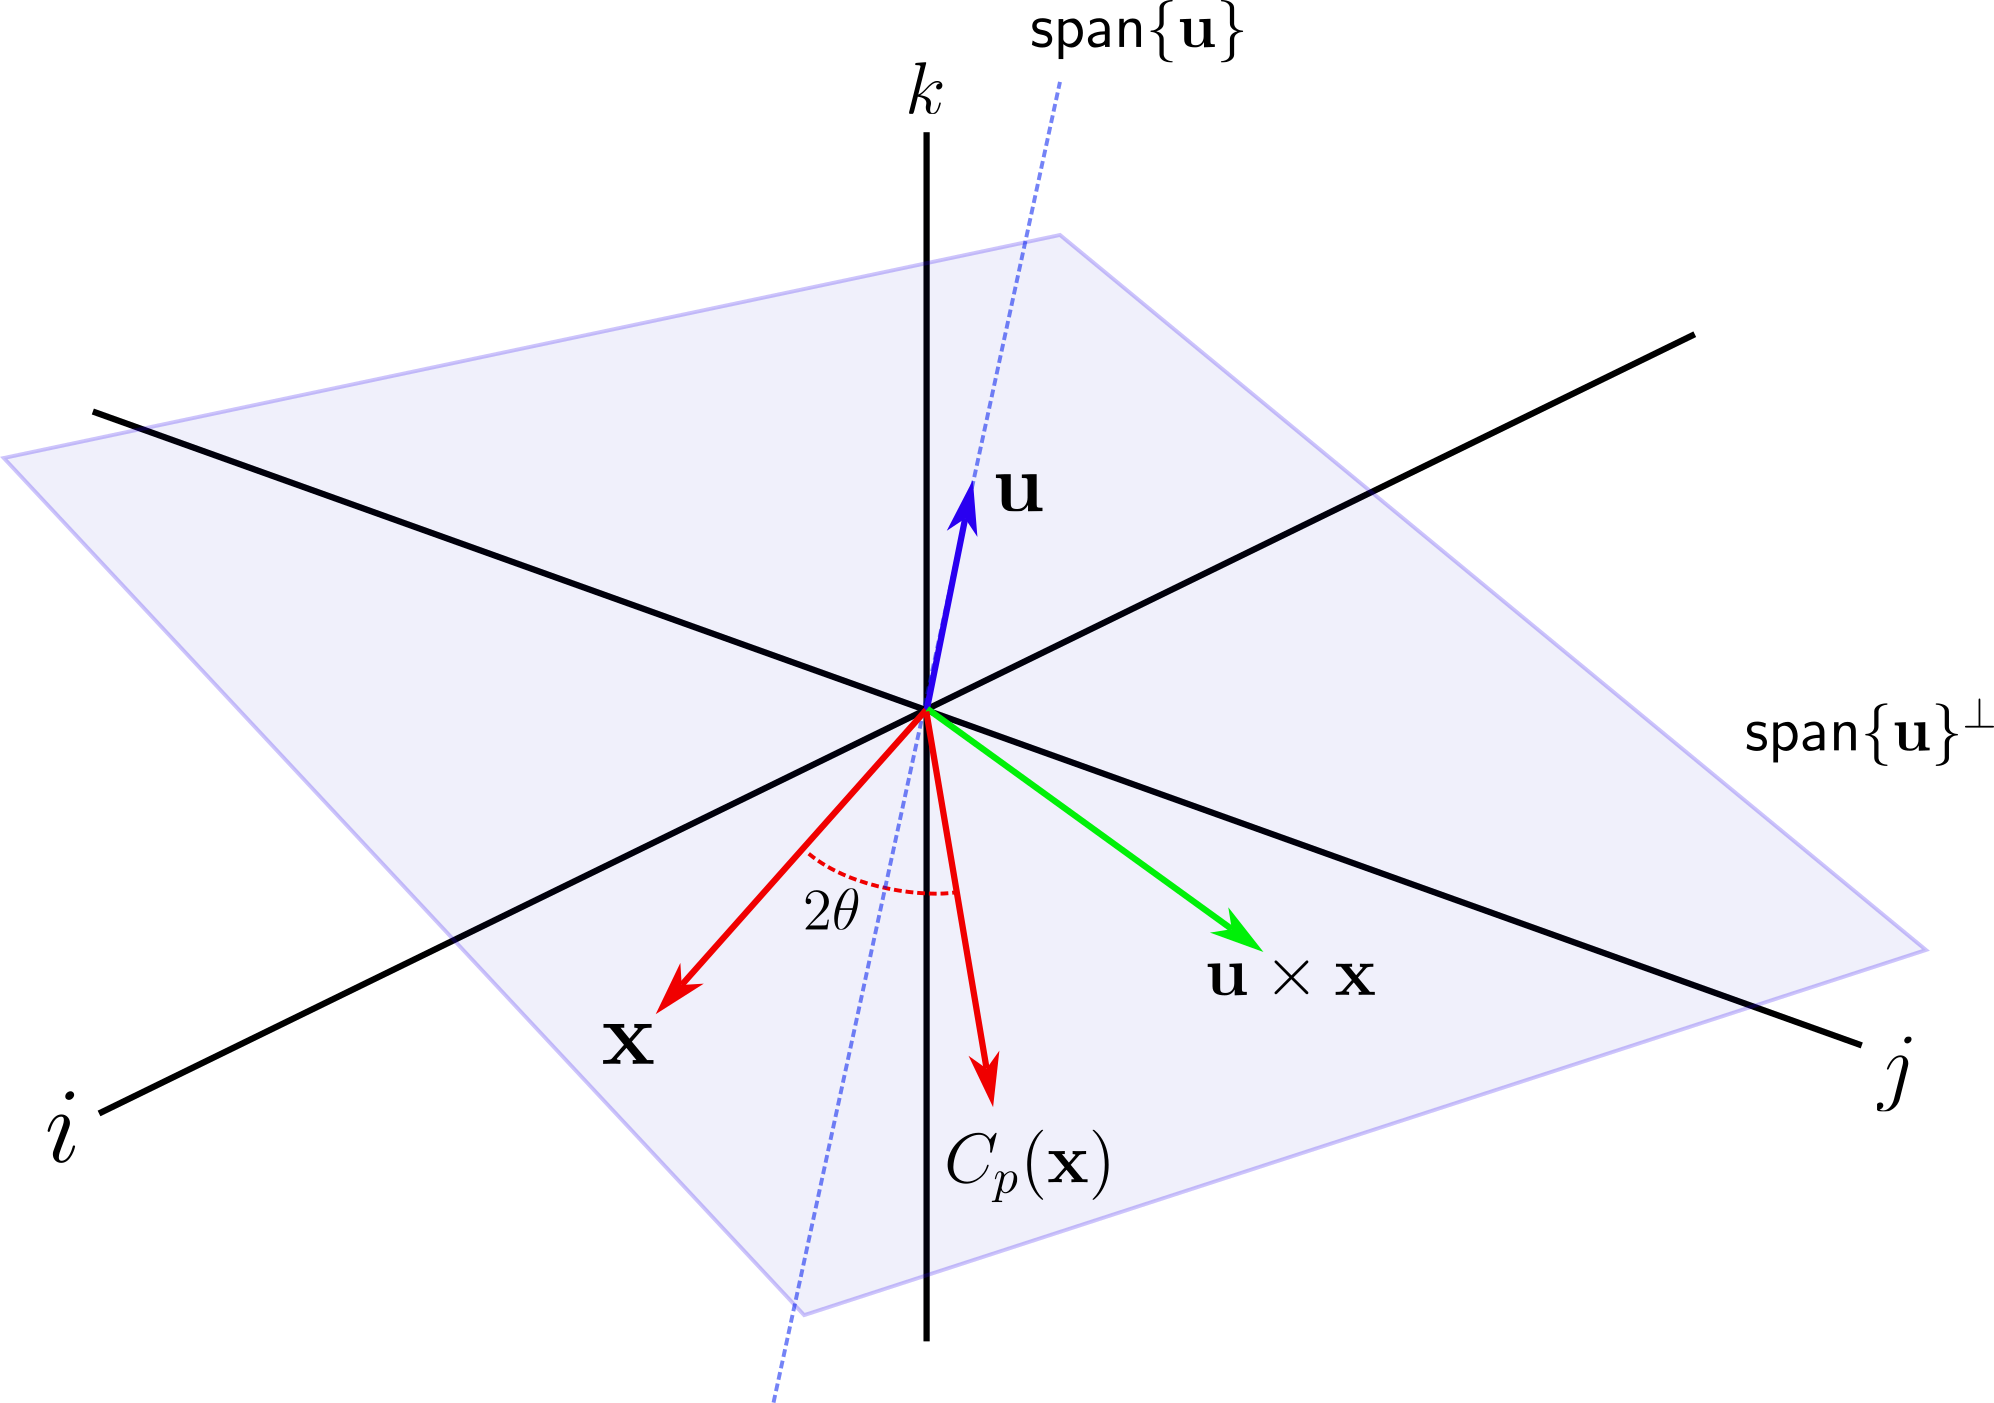
\includegraphics[width=0.8\linewidth]{quaternion.png}
    \caption{Diagram of rotation including the vectors $\vec{u},\vec{x},\vec{u}\times\vec{x}$.}
    \label{fig:quaternion}
\end{figure}

\subsubsection{Exact Sequences and Double Covers}
\begin{defn}[Exact Sequence]
Let $G_1,...,G_n$ be a list of groups, and suppose there are maps $f_0: \{1\} \to G_1, f_1 : G_1 \to G_2, ..., f_{n-1} : G_{n-1}\to G_n, f_n : G_n\to\{1\}$, where $\{1\}$ is the trivial group. That is, we have a diagram
\[1\to G_1\to\cdots \to G_n\to 1\]
Suppose these maps satisfy $\ker f_{i} = \image f_{i-1}$ for all $i=1,...,n+1$. Then we say the sequence $G_1,...,G_n$ forms an \textbf{exact sequence}.  
\end{defn}
\begin{example}
Observe that the set $\ZZ/2 = \{-1,1\}$ is a group with respect to multiplication.
Define \[f_0 : 1 \to \ZZ/2\] 
by $f_0(1) = 1$. Define
\[f_1 : \ZZ/2 \to S^3\] by $f_1(1) = 1, f_1(-1) = -1$. Define 
\[f_2 : S^3\to \SO(3,\RR)\] by $f_2(p) = C_p$, and define 
\[f_3 : \SO(3,\RR)\to 1\]
 by $f_3(R) = 1$. 

This gives us an exact sequence of maps,
\begin{equation}1\to \ZZ/2 \to S^3 \to \SO(3,\RR)\to 1\label{eq:so3exact}\end{equation}
\end{example}
\begin{defn}
Let $A,B,C$ be groups.
Let $\iota : A\to A\times C$ be given by $\iota(a)=(a,1)$, and let $p : A\times C \to C$ be given by $p(a,c) = c$. Suppose that we have an exact sequence,
\[1\to A\xrightarrow[a]{} B\xrightarrow[b]{} C \to 1\]

    Then we say this sequence \textbf{splits} if there exists an isomorphism $f : B\to A\oplus C$ so that $f\circ a = \iota$ and $p\circ f = b$. 
\end{defn}
\begin{thm}
The exact sequence \eqref{eq:so3exact} does not split. In other words, there does not exist any map $\varphi : \SO(3,\RR) \to S^3$ so that $\varphi \circ C = \One$.
\end{thm}
\begin{proof}
    Suppose $\varphi$ existed. Then $[S^3 :\image \varphi] = 2$, so $\image\varphi$ is a normal subgroup of $S^3$.

    By the first isomorphism theorem, this would mean $S^3/\image\varphi$ is isomorphic to $\ZZ/2$. Let $\rho : S^3 \to S^3/\image\varphi$ be the quotient map.

    Recall that if $u,v\in S^2$, there exists $r\in S^3$ so that $rvr^{-1} = u$. Since $\ZZ/2$ is abelian, we have $\rho(u)=\rho(rvr^{-1}) = \rho(v)$ for all $u,v\in S^2$.

    Now recall that a basis for $\HH$ is given by $\{e_0,e_1,e_2,e_3\}$. We have $\rho(e_3)=\rho(e_1)\rho(e_2)$, and since $u,e_1\in S^2$ we have $\rho(u) = \rho(e_1) = \rho(e_2)^{-1}\rho(e_3) = \rho(e_2^{-1}e_2)=1$. Therefore, $\rho(u)=1$ for all $u \in S^2$.

    Now, if $p \in S^3$, then recall that there exist $u,v\in S^2$ with $p=uv$. So $\rho(p) = 1$ as well. 

    But this means that $\rho$ is not surjective, since $\image \rho = \{1\} \neq S^3/\image\varphi$. This is a contradiction, so the proof is complete.
\end{proof}
\begin{remark*}
    We say that since this sequence does not split, and since $\ker C$ has two elements, the map $C : S^3\to \SO(3,\RR)$ is a \textbf{nontrivial double cover}.
\end{remark*}
\begin{remark*}
    As we will soon see, this is really a statement about the \textbf{spin group}, $\Spin(3) = S^3$.
\end{remark*}
Now we will return to the study of the map $K_{p,q}$. 
\begin{lemma}
    The sequence,
    \[1\to \ZZ/2\to S^3\times S^3 \xrightarrow[K]{} \to \SO(4,\RR) \to 1\]
    is exact.
\end{lemma}
\begin{proof}
    All we need is for $K$ to be surjective. 

    Topologically, we can see that since $\image K$ contains the identity, we must have $\image K \subseteq \SO(4,\RR)$.

    Furthermore, by Cartan-Dieudonn\'e theorem any $P$ in $\SO(4,\RR)$ can be written as $P = R_{u_{2m}}\circ...\circ R_{u_1}$, with each $u_i \in S^3$.

    Therefore since $K$ is a homomorphism, if we can show that $R_{u_2}\circ R_{u_1}\in \image K$ for all $u_1,u_2$ then it follows that $\SO(4,\RR) \subseteq \image K$.

    Suppose $u_1 = \pm u_2$. Then $R_{u_2}\circ R_{u_1}=\One$. So this case is done.

    Now suppose $u_1$ and $u_2$ are linearly independent. Let $u_1 = v_1$. Then there exists $v_2$ with $u_2 = \cos\theta v_1 + \sin\theta v_2$, where $\theta = \arccos(\langle u_1,u_2\rangle)$ is the angle between the two unit quaternions. Now let $x \in \RR^4$. We have,
    \begin{align*}
        R_{u_2}(R_{u_1}(x))&= x-2\langle x,u_1\rangle u_1 - 2(\langle x-2\langle x,u_1\rangle u_1,u_2\rangle)u_2
    \end{align*}
    Exercise: check that if $x \perp \Span\{u_1,u_2\}$ then $R_{u_2}(R_{u_1}(x))=x$, and if $x \in \Span\{u_1,u_2\}$ then $R_{u_2}(R_{u_1}(x))=\cos(2\theta)x+\sin(2\theta)v_3$ for some $v_3$.

    Finally we just need to show that any rotation of this form is in the image of $K$. Let $L = \Span\{u_1,u_2\}^\perp$. Then $\HH = L\oplus L^\perp$, where $P$ fixes $L$ and rotates $L^\perp$. This is done in two cases.

    First, if $1 \in L$ then $P$ must be in $\SO(3,\RR)$ and $P = K_{p,p}$ for some $P$.

    The other case: MISSING
 \end{proof}
\begin{remark*}
    This exact sequence does not split. That is, $S^3\times S^3 \to \SO(4,\RR)$ is a nontrivial double cover. We will soon see that this is a fact about spin groups, $S^3\times S^3 = \Spin(4)$.
\end{remark*}

\section{Clifford Algebras}
\subsection{Lecture 15: Clifford Algebras}
\subsubsection{Interior Product Revisited}
Recall that the interior product is defined by,
\[\hk : V\times \Lambda^k V^* \to \Lambda^{k-1} V^*\]
where,
\[v\hk\omega(u_1,...,u_{k-1}) = \omega(v,u_1,...,u_{k-1})\]
Given a metric $G$ and $a \in \Lambda^k V$, we can also set,
\[v\hk a(\alpha_2,...,\alpha_{k-1}) = a(\flat(v),\alpha_2,...,\alpha_{k-1})\]
\begin{remark*}
    Given this, we see that $v\hk v = G(v,v)$ for any $v \in V$. Therefore the interior product is a generalization of the inner product.
\end{remark*}
\begin{remark*}
    An explicit formula is given as follows. Let $\alpha = \alpha_1\wedge...\wedge\alpha_k$. Then,
    \begin{align*}v\hk\alpha(v_2,...,v_k) &=\alpha(v,v_1,...,v_{k-1})\\&= \sum_{\sigma\in S_k} \sgn(\sigma)\alpha_{\sigma(1)}(v)\alpha_{\sigma(2)}(v_2)...\alpha_{\sigma(k)}(v_k)\\
    &= \sum_{j=1}^k\sum_{\sigma\in S_{k},\sigma(1)=j} \sgn(\sigma)\alpha_{\sigma(1)}(v_1)\left(\alpha_{\sigma(2)}(v_2)...\alpha_{\sigma(k)}(v_k)\right)\\
    &= \sum_{j=1}^k (-1)^{j+1}\alpha_{j}(v_1)\sum_{\sigma\in S_{k-1}} \sgn(\sigma)\alpha_{i_{\sigma(1)}}(v_2)...\alpha_{i_{\sigma(k-1)}}(v_k) \intertext{Where  $i_1=2,...,i_{j-1} = j-1, i_{j}=j+1,...,i_{k-1}=k$.}\\
    &= \sum_{j=1}^k (-1)^{j+1}\alpha_{j}(v)\left(\alpha_1\wedge...\wedge\alpha_{j-1}\wedge\alpha_{j+1}\wedge...\wedge\alpha_k(v_2,...,v_k)\right)
    \end{align*}
    In other words,\begin{equation}
        v\hk\alpha = \sum_{j=1}^k (-1)^{j+1}\alpha_{j}(v)\;\alpha_1\wedge...\wedge\alpha_{j-1}\wedge\alpha_{j+1}\wedge...\wedge\alpha_k
    \end{equation}
    Here we have factored out the $\alpha_{\sigma(1)}(v)$ and set $j=\sigma(1)$. Then we can sum over $\sigma(1)$ separately from the other outputs, which effectively means we are summing over the permutations of $2,...,k$. Therefore we get the wedge product of all but $\alpha_{\sigma(1)}$ in the end. 
\end{remark*}
\begin{lemma}
    Let $v\in V$, $\alpha\in \Lambda^{p}V^*, \beta\in \Lambda^{q}V^*$. Then,
    \begin{equation}
        v\hk(\alpha\wedge\beta) = (v\hk \alpha)\wedge\beta + (-1)^p \alpha\wedge(v\hk\beta)
    \end{equation}
    In other words, the interior product is an \textbf{(anti)-derivation}. It obeys a ``graded" version of the Leibniz rule.
\end{lemma}
\begin{proof}
    By linearity it suffices to show this for wedge-decomposable forms. Let $\alpha = \alpha_1\wedge...\wedge\alpha_p$, $\beta = \beta_1\wedge...\wedge\beta_q$. 

    To make the proof easier, we will introduce the notation $\gamma_i = \alpha_{i},i=1,...,p$ and $\gamma_{i+k}=\beta_i,i=1,...,q$. This way, $\alpha = \gamma_1\wedge...\wedge\gamma_p$ and $\beta = \gamma_{p+1}\wedge...\wedge\gamma_{p+q}$    
    Then,
    \begin{align*}
        (v\hk\alpha)\wedge\beta &= \sum_{i=1}^p (-1)^{i+1}\gamma_i(v)\gamma_1\wedge...\wedge\gamma_{i-1}\wedge\gamma_{i+1}\wedge...\wedge\gamma_{p}\wedge\gamma_{p+1}\wedge...\wedge\gamma_{p+q}\\
        (-1)^{p}\alpha\wedge(v\hk\beta)&= (-1)^p\sum_{i=p+1}^{p+q}(-1)^{i+p+1}\gamma_i(v)\gamma_1\wedge...\wedge\gamma_p\wedge...\wedge\gamma_{i-1}\wedge\gamma_{i+1}\wedge...\wedge\gamma_{p+q}\\
        &=\sum_{i=p+1}^{p+q}(-1)^{i+1}\gamma_i(v)\gamma_1\wedge...\wedge\gamma_p\wedge...\wedge\gamma_{i-1}\wedge\gamma_{i+1}\wedge...\wedge\gamma_{p+q}
    \end{align*}
    Adding these together, we get,
    \[(v\hk\alpha)\wedge\beta+(-1)^{p}\alpha\wedge(v\hk\beta)=\sum_{i=1}^{p+q}(-1)^{i+1}\gamma_i(v)\gamma_1\wedge...\wedge\gamma_{i-1}\wedge\gamma_{i+1}\wedge...\wedge\gamma_{p+q}\]
    The right hand side is exactly $v\hk(\alpha\wedge\beta)$ as required.
\end{proof}
\begin{thm}
Let $G$ be a metric on $V$.
    Let $v\in V,\alpha\in\Lambda^{k-1}V, \beta\in\Lambda^k V$. Then,
    \begin{equation}
        G(v\wedge \alpha,\beta) = G(\alpha,v\hk \beta)
    \end{equation}
    In other words, the interior product is the \textbf{adjoint} of the exterior product.
\end{thm}
\begin{proof}
    By linearity it is enough to show that this is true for wedge-decomposable forms. Let $\alpha = \alpha_2\wedge...\wedge \alpha_{k-1}$, $\beta = \beta_1\wedge...\wedge \beta_k$. Then we have,
    \begin{align*}
        G(v\wedge\alpha,\beta) &= G(v\wedge\alpha_2\wedge...\wedge \alpha_{k-1},\beta_1\wedge...\wedge \beta_{k})\\
        &= \det\m{G(v,\beta_1)&\cdots & G(v,\beta_k)\\
        \vdots &\ddots&\vdots\\
        G(\alpha_k,\beta_1)&\cdots&G(\alpha_k,\beta_k)}\\
        &= \sum_{j=1}^k (-1)^{j+1}G(v,\beta_j)\det [G(\alpha_i,\beta_j)]_{i\neq j}\\
        &=\sum_{j=1}^k (-1)^{j+1}G(v,\beta_j)\beta_1\wedge...\wedge\beta_{j-1}\wedge\beta_{j+1}\wedge...\wedge\beta_k(\alpha_2,...,\alpha_{k-1})\\
        &=v\hk\beta(\alpha_2\wedge...\wedge\alpha_{k-1})\\
        &= G(\alpha,v\hk\beta)
    \end{align*}
    Where in line 3 we have used the cofactor expansion to sum over the first row of the overlap matrix, and from line 4 to 5 we have used the formula for the interior product derived above.
\end{proof}
\begin{lemma}
Let $G$ be a metric on $V$.
Let $w\in V$ and $\alpha\in \Lambda^k V$. Then,
\begin{equation}
    w\hk (w\wedge\alpha) = |w|^2\alpha
\end{equation}
\label{lemma:15.2}
\end{lemma}
\begin{proof}
    By the product rule for the interior product we have $w\hk(w\wedge \alpha) = (w\hk w)\wedge\alpha - w\wedge(w\hk\alpha)$. We know $w\hk w = w(\flat(w)) = G(w,w)$. So $(w\hk w)\wedge \alpha = |w|^2\alpha$.
    
    
    Therefore we just need to show that the second term vanishes. We have,
    
    \begin{align*}w\wedge(w\hk\alpha)(v_1,...,v_{k})&=\left[w\wedge \sum_{j=1}^k (-1)^{j+1}\alpha_j(w) \alpha_1\wedge...\wedge\alpha_{j-1}\wedge\alpha_{j+1}\wedge...\wedge\alpha_k\right](v_1,...,v_{k})\\
    &=\left[\sum_{j=1}^k \alpha_j(w) \alpha_1\wedge...\wedge\alpha_{j-1}\wedge w\wedge \alpha_{j+1}\wedge...\wedge\alpha_k\right](v_1,...,v_{k})\end{align*}
\end{proof}
\begin{defn}
    We define the following notation.

    Let $I_v : \Lambda^k V \to \Lambda^{k-1}V$ be given by $I_v(\alpha) = v\hk \alpha$, and let $E_v : \Lambda^k V \to \Lambda^{k-1}V$ be given by $E_v(\alpha) = v\wedge \alpha$.
\end{defn}
\begin{remark*}
    Note that $E_v^2 = I_v^2 = 0$.
\end{remark*}
\begin{cor}
    In the proof of lemma \ref{lemma:15.2} we showed that $I_v \circ E_v + E_v\circ I_v = \langle v,v\rangle\One$.
\end{cor}
\subsubsection{Quotient Algebras}
Here we will first go over the definition of a quotient algebra. The definition is almost the same as a quotient vector space, except in order for the quotient to form an algebra we will require that the denominator is more than just a vector space. We will require that it is an ideal.
\begin{defn}[Ideal of an Algebra]\index{Algebra!Ideal}\index{Ideal!Algebra}
    Let $A$ be an algebra. Then an \textbf{ideal} is a vector subspace $B$ of $A$ with the additional property that if $v\in A$ and $w \in B$ then $vw \in B$ and $wv\in B$.

    In other words, an ideal is a vector subspace which \textit{absorbs vector multiplication from the left and right}.
\end{defn}
\begin{defn}
    Let $A$ be an algebra and let $B$ be an ideal of $A$. Then the \textbf{quotient algebra} is the set of equivalence classes $[v] = \{v + b : b \in B\}$, and is denoted,
    \[A/B = \{[v] : v\in A\}\]
    Sometimes we use the notation $[v] = v+B$.
\end{defn}
\begin{remark*}
    Observe that since $B$ is an ideal, we have $wB = Bw = B$ for all $w\in A$, and $B^2 = \{bB : b \in B\} = B$, by the absorption property. Therefore,
    \[[v][w] = (v+B)(w+B) = vw+vB+wB+BB = vw + B = [vw]\]
    This means that the quotient of an algebra by an ideal is indeed a well defined algebra, and the multiplication rule from the original algebra still makes sense.
\end{remark*}

\subsubsection{The Clifford Algebra}

Recall definition \ref{defn:tensoralgebra} of the \textbf{tensor algebra}. It is given by 
\[\bigotimes V = \bigoplus_{k=0}^\infty V^{\otimes k}\]
Each element of $\bigotimes V$ is of the form $\sum_{k=0}^N Y_k$ with each $Y_k \in V^{\otimes k}$. 
\begin{example}
    Let $V = \RR^3$. Then, for example,
    \[1 + e_1 + 3e_1\otimes e_2 \otimes e_3 \in \bigotimes V\]
\end{example}
\begin{remark*}
    The set $\bigotimes V$ is a real algebra, where multiplication is given by the tensor product. The subset $\RR \subseteq \bigotimes V$ forms a subalgebra.
\end{remark*}

\begin{defn}
Let $V$ be a vector space with a metric $G(v,w)$ which we denote by $G(v,w) = \langle v,w\rangle$. The \textbf{Clifford ideal} of $V$ is the set
    \[I(V)=\left\{\sum_{k=1}^N \alpha_k \otimes(v_k\otimes v_k+\langle v_k,v_k\rangle 1)\otimes \beta_k: \quad \alpha_k,\beta_k \in \bigotimes V, v_k\in V\right\}\]
    That is, $I(V)$ is the \textbf{ideal} generated by elements of the form $v\otimes v+\langle v,v\rangle1$. 
\end{defn}
\begin{defn}[Clifford Algebra]\index{Algebra!Clifford Algebra}
Let $V$ be a vector space and let $G$ be a metric on $V$. Then the \textbf{Clifford algebra} of $V$ is the quotient,
    \begin{equation}
        \Cl(V,G) = \frac{\bigotimes V}{I(V)}
    \end{equation}
It is associative.
\end{defn}
\begin{remark*}
    The multiplication is denoted $\alpha \cdot \beta = [\alpha\otimes\beta] = \alpha\otimes\beta + I(V)$.
\end{remark*}
\begin{thm}
Let $v,w \in \Cl(V,G)$. Then,
    \begin{equation}
        v\cdot w + w\cdot v = - 2G(v,w) = -2\langle v,w\rangle
    \end{equation}
    And in particular, 
    \begin{equation}
        v\cdot v = -Q(v)=-|v|^2
    \end{equation}
\end{thm}
\begin{proof}
    Note that $(v+w)\otimes (v+w) + |v+w|^21 
 \in I(V)$ for all $v,w$. We can rewrite this to derive another identity.
    We have,
    \begin{align*}
        (v+w)\otimes (v+w) + |v+w|^21&= v\otimes w + |v|^21 +v\otimes v +  w\otimes v + |w|^21 + \langle v,w\rangle1 + \langle w,v\rangle1\\
        &= v\otimes w + w\otimes v + 2\langle v,w\rangle1 + (v\otimes v+|v|^21) + (w\otimes w+|w|^21)
    \end{align*}
    Since $v\otimes v + |v|^21$ and $w\otimes w+|w|^21$ are both elements of $I(V)$, and $I(V)$ is closed under addition,
    \[(v+w)\otimes (v+w) + |v+w|^21-v\otimes v + |v|^21-w\otimes w+|w|^21 \in I(V)\]
    Therefore, $v\otimes w + w\otimes v + 2\langle v,w\rangle \in I(V)$. In other words,
    \[
        v\cdot w + w\cdot v + 2\langle v,w\rangle = [v\otimes w + w\otimes v + 2\langle v,w\rangle1] = [0] = 0
    \]
    This completes the proof.
\end{proof}
\subsubsection{Universal Properties}
A \textbf{universal property} is a feature of a set which completely characterizes it. Before covering the universal property of the Clifford algebra, I figured it would be good to show some simpler examples.
\begin{defn}[Universal Property] \index{Universal Property!Definition}
    A property of a set $S$ with some structure (such as a group, algebra, vector space, etc structure) is called a \textbf{universal property} if any other set with the same property is isomorphic (in the sense of the aforementioned structure) to $S$.
\end{defn}

\begin{example}[Universal Property of the Product]\index{Universal Property!Products}
Let $A$ and $B$ be sets. Recall that, given the product $A\times B$, there are maps $\pi_A : A\times B \to A$ with $\pi_A(a,b)=a$, and $\pi_B : A\times B \to B$ with $\pi_B(a,b) =b$.

The universal property which completely characterizes $A\times B$ is as follows. Consider the following diagram.
\begin{center}
\begin{tikzcd}
  & D \arrow[d, "\phi"'] \arrow[ldd, "f_1"'] \arrow[rdd, "f_2"] &   \\
  & C \arrow[ld, "\pi_X"] \arrow[rd, "\pi_Y"']                  &   \\
A &                                                             & B
\end{tikzcd}
\end{center}

Suppose $C$ is a set and that there exist surjective functions $\pi_A : C\to A$ and $\pi_B : C \to B$.  

We say that $C$ is satisfies the \textbf{universal property} of $A\times B$ if for all sets $D$, and functions $f_1 : D\to A, f_2 : D \to B$, there exists a unique function $\phi : D \to C$ so that $f_1 = \pi_A\circ \phi$ and $f_2 = \pi_B \circ \phi$.

If two sets $C_1$ and $C_2$ obey the universal property, then $C_1$ and $C_2$ are in bijection. Therefore, we denote $C = A\times B$, since any two sets satisfying the universal property are essentially the same.

If we put more requirements on the arrows in the diagram, we end up with the equivalent of the cartesian product for different kinds of special sets.

For example, if $A,B,C,D$ are taken to be groups, and all the functions in the diagram are group homomorphisms, then the above universal property says that $C = A\times B$ if and only if for all groups $D$ and group homomorphisms $f_1:D\to A,f_2:D\to B$, there exists a group isomorphism $\phi : D \to C$ satisfying the equations $f_1 = \pi_A\circ\phi$ and $f_2=\pi_B\circ\phi$. 

Similarly we can construct the equivalent of the product for vector spaces, algebras and so on.
\end{example}
\begin{thm}[Universal Property of the Clifford Algebra]\index{Universal Property!Clifford Algebra}
    Let $V$ be a vector space over $\RR$ and let $A$ be a unital algebra over $\RR$. 

    Suppose that $\phi : V \to A$ is a linear map, and suppose $\phi(x)\phi(x) = -G(x,x)1_A$ for all $x \in V$.

    Suppose $B$ is an algebra, and that there exists an injective linear map $\iota : V \to B$, and a unique algebra homomorphism $\tilde{\phi}:B\to A$ so that $\tilde{\phi}\circ\iota =\phi$. Then there is an algebra isomorphism between $B$ and the Clifford algebra of $V$.

    That is, $B\cong \Cl(V,G)$ iff for all unital associative algebras $A$ and all linear maps $\phi : V\to A$ with $\phi(x)\phi(x)=-G(x,x)1_A$, there exists a unique diagram
    \begin{center}
\begin{tikzcd}
V \arrow[d, "\iota"'] \arrow[r, "\phi"] & A \\
B \arrow[ru, "\tilde{\phi}"']           &  
\end{tikzcd}
    \end{center}
    Where $\iota$ is injective, $\tilde{\phi} = \phi\circ\iota$, and $\tilde{\phi}$ is a homomorphism.
\end{thm}
\begin{proof}
    We must first show that $\bigotimes V/I(V)$ satisfies this property, and then show that if $B$ satisfies the same property then $B\cong \bigotimes V/I(V)$.

    Let $\phi:V\to A$ be a linear map. 
    
    First note that any algebra homomorphism $g : \bigotimes V \to A$ must satisfy the formula, $g(v_1\otimes...\otimes v_k) = g(v_1)...g(v_k)$.

    We then define an algebra homomorphism $\hat{\phi} : \bigotimes V \to A$  by the formula $\hat{\phi}(v_1\otimes...\otimes v_k) = \phi(v_1)...\phi(v_k)$ for all $v_1,...,v_k$, and then extend it by linearity. 
    
    We can see that $\hat{\phi}(v)=\phi(v)$, so $\hat{\phi}|_{V} = \phi\circ\iota_0$, where $\iota_0 : V \to \bigotimes V$ is the inclusion map.

    Suppose that we had any other algebra homomorphism $g : \bigotimes V \to A$ which satisfied $g|_V = \phi\circ \iota_0$. Then we would have $g(v) = \phi(v)$, so 
    \begin{align*}\hat{\phi}(v_1\otimes...\otimes v_k) &= \phi(v_1)...\phi(v_k) \\&= g(v_1)...g(v_k)\\&=g(v_1\otimes ...\otimes v_k)\end{align*}
    By linearity, we see that $\hat{\phi} = g$. Therefore $\hat{\phi}$ is unique.

    Since $\phi(x)\phi(x) = -|x|^21$, we have $\phi(x\otimes x + |x|^21) = 0$. Therefore $I(V) \subseteq \ker \phi$. Let $q : \bigotimes V \to \bigotimes V/I(V)$ be the quotient map, and let $\tilde{\phi} : \bigotimes V/I(V) \to A$ be given by $\tilde{\phi}(v_1...v_k) = \phi(v_1)...\phi(v_k)$. Then since $\ker \phi$ contains $I(V)$ we have $\tilde{\phi} = q\circ \hat{\phi}$. Since $\hat{\phi}$ is unique, $\tilde{\phi}$ is the unique extension of $\phi$ to $\Cl(V)$. That is, we have shown that $\bigotimes V/I(V)$ satisfies the universal property of $\Cl(V)$. This completes the proof of the first half.

    Now we must prove that if $A$ is any other algebra which satisfies the universal property of the Clifford algebra, then $A$ is isomorphic to $\bigotimes V/I(V)$.

    First, we have that any linear map $\varphi : V \to A$ with $\phi(x)\phi(x) = -|x|^2$ has a unique extension to an algebra homomorphism $\varphi : \Cl(V)\to A$.
\end{proof}
\begin{cor}
    Let $\{e_1,...,e_n\}$ be an orthonormal basis for $V$. That is, $\langle e_i,e_j\rangle=\pm\delta_{ij}$. Suppose $\varphi : V \to A$ satisfies $\varphi(e_j^2) = -|e_j|^2$ and $\varphi(e_i)\varphi(e_j)+\varphi(e_j)\varphi(e_i)=0$. Then $\varphi$ has a unique extension to $\varphi : \Cl(V)\to A$.
\end{cor}
\begin{proof}
    We have $\varphi(e_i\otimes e_i + |e_i|^21) = 0$ by definition. Using the polarization identity and linearity, one can expand each term in $x\otimes y + y \otimes x + 2\langle x,y\rangle 1$ in terms of a basis, before applying $\varphi$ to show that $\varphi(x)\varphi(y)+\varphi(y)\varphi(x)=-2\langle x,y\rangle 1$. So $\ker \varphi$ contains $I(V)$. This completes the proof.
\end{proof}
\begin{thm}
    The vector space $\Lambda^\bullet V$ is canonically isomorphic as a vector space to $\Cl(V)$.

    Furthermore, if $v,w \in \Cl(V)$, then $vw = v\wedge w -v\hk w$.
\end{thm}
We will delay the proof until after some remarks.
\begin{remark*}
    Let $\phi : \Lambda^\bullet V\to \Cl(V)$ be the canonical isomorphism. Let $\iota : V \to \Cl(V)$ be the inclusion map. Then $\iota\circ \phi$ is injective.
\end{remark*}
\begin{remark*}
    It is not isomorphic as an algebra to $\Cl(V)$ because they have different multiplications.
\end{remark*}
\begin{defn}[Clifford Product]
    When we interpret elements $v,w$ of $\Cl(V)$ as elements of $\Lambda^\bullet V$, the product $vw$ is referred to as the \textbf{Clifford product}.
\end{defn}
\begin{remark*}
    The Clifford algebra is not a graded algebra (recall Definition \ref{defn:gradedalgebra}) since the Clifford product of two $k$-forms is not a $k+\ell$-form.
\end{remark*}
\begin{remark*}
    Some books define $\Cl(V)$ to be generated by the ideal $I(V) = \langle v\otimes v - |v|^21\rangle$ instead, in which case the Clifford product is $vw = v\wedge w + v\hk w$. This is equivalent to replacing the metric $G$ with $-G$, or replacing the signature $(p,q)$ with $(q,p)$.
\end{remark*}
Now we will get to the proof of the theorem.
\begin{proof}
    We first show that the restriction of the quotient map $q : \bigotimes V \to \Cl(V)$ to the subspace $\Lambda^\bullet V \subset\bigotimes V$ is surjective. That is, every equivalence class can be represented by a skew-symmetric tensor.

    For a tensor of degree $0$ or $1$ this is trivial. Let $\beta\in \bigotimes V$ be decomposable. Then 
    \[\beta = \frac{1}{2}(x\otimes y + y \otimes x) + \frac{1}{2}(x\otimes y - y\otimes x)\]
    Adding and subtracting $G(x,y)1$, we can get this to be in the form
    \[\beta=\frac{1}{2}(x\otimes y+y\otimes x+2G(x,y)1)-G(x,y)1\]
    Where the first term is an element of $I(V)$ and the second term is an element of $\Lambda^0 V$.

    Inductively we can show that any decomposable $k$-tensor can be written as something in $I(V)$ plus something in $\Lambda^0 V$.

    We have a surjection from $\Lambda^\bullet V$ to $\Cl(V)$. Now we need to construct a surjection from $\Cl(V)$ to $\Lambda^\bullet V$. 

    We will use the universal property to construct a map $\varphi : V \to \mathsf{End}(\Lambda^\bullet V)$. First we remark that $\mathsf{End}(\Lambda^\bullet V)$ is an algebra over $\RR$ with identity. Then set $\varphi(x) = [E_x - I_x]$ for $x \in V$. Then $\varphi(v)(w)=v\wedge w - w\wedge v$ and so $\varphi(v)\circ\varphi(w)=[E_x-I_x]^2=-|x|^2\One$. So $\varphi$ extends uniquely to an algebra homomorphism $\varphi : \Cl(V) \to \mathsf{End}(\Lambda^\bullet V)$.

    Now let us define $\psi : \mathsf{End}(\Lambda^\bullet V) \to \Lambda^\bullet V$ by $\psi(A) = A(1)$. Observe that this map is linear. Let us define $L = \frac{1}{k!}\psi\circ \varphi : \Cl(V) \to \Lambda^\bullet V$, which is linear.

    Let $\alpha = v_1\wedge...\wedge v_k \in \Lambda^\bullet V$. We have
    \begin{align*}
        L\circ q(\alpha) &= L([\alpha])\\
        &= L([v_1\wedge...\wedge v_k])\\
        &= L\left(\left[\sum_{\sigma \in S_k} \sgn(\sigma)\;v_{\sigma(1)}\otimes...\otimes v_{\sigma(k)}\right]\right)\\
        &= L\left(\sum_{\sigma \in S_k} \sgn(\sigma)\;v_{\sigma(1)}... v_{\sigma(k)}\right)\\
        &= \frac{1}{k!}\psi\circ\varphi\left(\sum_{\sigma \in S_k} \sgn(\sigma)\;v_{\sigma(1)}... v_{\sigma(k)}\right)\\
        &= \frac{1}{k!}\psi\left(\sum_{\sigma \in S_k} \sgn(\sigma)\;(E_{v_{\sigma(1)}}-I_{v_{\sigma(1)}})...(E_{v_{\sigma(k)}}- I_{v_{\sigma(k)}})\right)\\
        &= \frac{1}{k!}\sum_{\sigma \in S_k} \sgn(\sigma)\;(E_{v_{\sigma(1)}}-I_{v_{\sigma(1)}})...(E_{v_{\sigma(k)}}- I_{v_{\sigma(k)}})(1)\\
        &= \frac{1}{k!}\sum_{\sigma \in S_k} \sgn(\sigma)\;(E_{v_{\sigma(1)}}-I_{v_{\sigma(1)}})...(E_{v_{\sigma(k-1)}}- I_{v_{\sigma(k-1)}})(v_{\sigma(k)})
        \intertext{Note that $(E_{v_{\sigma(k-1)}}- I_{v_{\sigma(k-1)}})(v_{\sigma(k)})=v_{\sigma(k-1)}\wedge v_{\sigma(k)}-G(v_{\sigma(k-1)},v_{\sigma(k)})$. In the above sum, the term $(v_{\sigma(k-1)},v_{\sigma(k)})$ will always appear twice, with opposite signs. Since $G$ is symmetric, this means all the scalar terms vanish.}
        &= \frac{1}{k!}\sum_{\sigma \in S_k} \sgn(\sigma)\;v_{\sigma(1)}\wedge...\wedge v_{\sigma(k)} \\
        &= v_1\wedge...\wedge v_k
    \end{align*}
    Therefore, $L\circ q$ is an isomorphism. Since $q$ is surjective, this means $L$ has to be injective. Therefore, we have an injection $L : \Lambda^\bullet V \to \Cl(V)$.

    Finally, we have $\varphi(x\alpha) = \varphi(x)\varphi(\alpha)$, so $\psi(\varphi(x\alpha))=\varphi(x\alpha)1 = \varphi(x)\psi(\varphi(\alpha))$. So $L(x\alpha) = x\wedge L(\alpha) - x\hk L(\alpha)$. Therefore, for any $x \in V, \alpha \in \Lambda^\bullet V$ we know that $L$ maps $x\alpha$ to $x\wedge \alpha - x \hk \alpha$. We also know 
    \begin{align*}
        q\circ L(v_1...v_k)&=q(v_1\wedge...\wedge v_k)\\
        &= v_1...v_k
    \end{align*}
    So $q \circ L = \One$ and $L\circ q = \One$. This means $q=L^{-1}$. In other words, $L$ is an isomorphism.
\end{proof}
\begin{remark*}
    We can therefore just think of $\Cl(V)$ as the vector space $\Lambda^\bullet V$ along with the new multiplication rule $v\alpha = v\wedge \alpha - v\hk \alpha$ for $v\in V$ and $\alpha\in \Lambda^\bullet V$.
\end{remark*}
\begin{example}
    If $\alpha = 1$ then $v\alpha = v$.

    If $v,w\in V$ then $vw = v\wedge w - \langle v,w\rangle 1$.

    If $v,w,u \in V$ then 
    \begin{align*}u(vw) &= u(v\wedge w-\langle v,w\rangle 1)\\ &= u\wedge v \wedge w - \langle v,w\rangle u - u\hk v \wedge w + u \hk \langle v,w\rangle 1\\
    &= u\wedge v \wedge w - \langle v,w\rangle u - \langle u,v\rangle w + \langle u,w\rangle v\end{align*}
\end{example}

The Clifford algebra has a lot of extra structure, such as involutions, automorphisms, and anti-automorphisms. Also, a special case of the universal property is when $A$ is also a Clifford algebra.

\begin{thm}
    Let $V_1,G_1$ and $V_2,G_2$ be two vector spaces with metrics. Then for each isometry $P : V_1\to V_2$ we have a unique extension to an algebra homomorphism $\Cl(V_1)\to \Cl(V_2)$. 
\end{thm}
\begin{proof}
    We have $P(x)P(x) = -|P(x)|^2 1 = -|x|^2 1$. So $P$ satisfies the universal property.
\end{proof}

\begin{remark*}
    Each linear map $T : V_1 \to V_2$ has a unique extension to an algebra homomorphism $T : \Lambda^\bullet V_1 \to \Lambda^\bullet V_2$ (given by the exterior power). This extension is the same as the extension to a map $\Cl(V_1)\to \Cl(V_2)$ as long as $T$ preserves the metric.
\end{remark*}
\begin{remark*}
    If $Q : V_2 \to V_3$ is another isometry then $Q\circ P$ is an isometry and has a unique extension to a map $\tilde{Q\circ P} :\Cl(V_1)\to \Cl(V_3)$. It is equal to $\tilde{Q}\circ\tilde{P}$.
\end{remark*}

\begin{defn}
    Let $\Aut_{\textsf{alg}}(\Cl(V))$ denote the set of all algebra automorphisms of $\Cl(V)$.

    The set of \textbf{Clifford automorphisms} is the set of all automorphisms which map $V$ into $V$, and is denoted $\Aut(\Cl(V))$.\index{Automorphism!Clifford Automorphism}
\begin{equation}
    \Aut(\Cl(V)) = \{P \in \Aut_{\textsf{alg}}(\Cl(V)) | P(V)\subseteq V\}
\end{equation}
\end{defn}

\begin{thm} The set of Clifford automorphisms of $V$ is equal to the orthogonal group of $V$. In other words $\Aut(\Cl(V)) = \Orth(V)$.
\end{thm}
\begin{proof}
    Suppose $P \in \Orth(V)$. Then $P$ maps $V$ to $V$ and preserves the inner product. Therefore, $P$ extends to a map $\Cl(V) \to \Cl(V)$, and since $P$ is invertible the extension is invertible. So $P$ is a Clifford automorphism.

    Now suppose $P \in \Aut(\Cl(V))$. Then \begin{align*}\langle P(x),P(x)\rangle &= -P(x)P(x) \\&= -P(x^2) \\&= P(-x^2) \\&= P(\langle x,x\rangle 1) \\&= \langle x,x\rangle\end{align*}
    So $P \in \Orth(V)$.

    Therefore every Clifford automorphism is an extension of an isometry of $V$.
\end{proof}
\subsubsection{Clifford Involutions}
We will now see that $\Cl(V)$ comes equipped with a special Clifford automorphism and two anti-automorphisms.

\begin{defn}[Canonical Clifford Automorphism]
    The isometry $P(v) = -v$ extends to an automorphism of $\Cl(V)$. We will denote the extension by the tilde symbol, so $\tilde{P}(\alpha) = \tilde{\alpha}$. It is called the canonical Clifford automorphism. Notice that $-(-v)=v$, so $\tilde{\tilde{v}}=v$. So the canonical automorphism is an involution.
\end{defn}
\begin{defn}[Even/Odd parts of the Clifford Algebra]
    The even/odd parts of the Clifford algebra are defined by,
    \begin{align}
        \Cl^{\textsf{even}}(V) &=\{\alpha \in \Cl(V) : \tilde{\alpha}=\alpha\}
        \\
        \Cl^{\textsf{odd}}(V) &=\{\alpha \in \Cl(V) : \tilde{\alpha}-=\alpha\}
    \end{align}
\end{defn}
\begin{lemma}
    Since $\alpha = \frac{1}{2}(\alpha+\tilde{\alpha}) + \frac{1}{2}(\alpha-\tilde{\alpha})$ we have
    \[\Cl(V) = \Cl^{\textsf{even}}(V)\oplus \Cl^{\textsf{odd}}(V)\]
\end{lemma}
Recall that $\Lambda^\bullet V$ is a graded algebra, and we have $\Lambda^\bullet V = \Lambda^{\textsf{even}}V\oplus \Lambda^{\textsf{odd}}V$, where $\Lambda^{\textsf{even}}V = \bigoplus \Lambda^{2k}V$ and $\Lambda^{\textsf{odd}}V = \bigoplus \lambda^{2k+1}V$.
\begin{lemma}
There exists vector space isomorphisms $\Lambda^{\textsf{even}}V \cong \Cl^{\textsf{even}}(V)$ and $\Lambda^{\textsf{odd}}V \cong \Cl^{\textsf{odd}}(V)$.
\end{lemma}
\begin{proof}
    Let $\{e_1,...,e_n\}$ be an orthonormal basis. Then $e_{i_1}...e_{i_k} = e_{i_1}\wedge...\wedge e_{i_k}$ since $e_{i_j}\hk e_{i_\ell}=0$ for all $j,\ell$. This means $\bigtilde{e_{i_1}...e_{i_k}} = \tilde{e}_{i_1}...\tilde{e}_{i_k} = (-1)^k e_{i_1}...e_{i_k}$. So the parity of the form $\alpha = e_{i_1}...e_{i_k}$ with respect to the canonical automorphism is the same as the parity of $\alpha$ with respect to the grading on $\Lambda^k V$. Extending by linearity completes the proof.
\end{proof}
\begin{defn}[Canonical Anti-Automorphism]
Consider the map $T : \bigotimes V \to \bigotimes V$ defined by,
\[T(v_1\otimes...\otimes v_k) = v_k\otimes v_{k-1}\otimes...\otimes v_2\otimes v_1\]
That is, it reverses the order of all components. This map is clearly an involution, and we can also see that it is an anti-automorphism with respect to the tensor product since $T(\alpha\otimes \beta) = T(\beta)\otimes T(\alpha)$. We write $T(\alpha) = \bigcheck{\alpha}$.
\end{defn}

\subsection{Lecture 16: Symmetries and Automorphisms of Clifford Algebras}
\subsubsection{Clifford Involutions (Continued)}
\begin{lemma}
Let $T(\alpha) = \bigcheck{\alpha}$ and $P(\alpha) = \bigtilde{\alpha}$. Then $T\circ P \circ T$ is an automorphism. Furthermore, since $(T\circ P \circ T)|_V = P|_V$, by uniqueness we see that $T\circ P \circ T = P$.  
\end{lemma}
\begin{defn}[Hat Anti-Automorphism]
    Let $T(\alpha) = \bigcheck{\alpha}$ and $P(\alpha) = \bigtilde{\alpha}$. Then we define $\bighat{\alpha} = T(P(\alpha))$. 
\end{defn}
\begin{remark*}
    By the above lemma, $T(P(\alpha))=P(T(\alpha))$. That is, $\bighat{\alpha}=\bigcheck{\bigtilde{\alpha}}=\bigtilde{\bigcheck{\alpha}}$.
\end{remark*}
\begin{thm}
    Let $a \in \Cl(V)$ be of degree $k$. Then $\bigtilde{a}=\pm a,$ $ \bigcheck{a}=\pm a,$ $\bighat{a}=\pm a$, where the signs are determined by $k$ according to the following table,
    \begin{center}
    \begin{tabular}{c|cccc}
         $k\mod 4$ & 0 &1&2&3  \\\hline
         $\sim$& +&-&+&-\\
         $\vee$&+&+&-&-\\
         $\wedge$&+&-&-&+
    \end{tabular}
    \end{center}
    \label{thm:kmod4}
\end{thm}
\begin{proof}
    Write down an orthonormal basis, and check directly.
\end{proof}
These involutions we have discussed have some important properties with respect to the metric induced on $\Cl(V)$ by the metric on $V$.
\begin{remark*}
Recall that the metric $G$ on $V$ induces a metric on $\Lambda^\bullet V$ (see equation \ref{eq:defn_induced_metric}). Since $\Lambda^\bullet V \cong \Cl(V)$ as vector spaces, we therefore also have a metric on $\Cl(V)$.
\end{remark*}
\begin{remark*}
    If $\{e_1,...,e_n\}$ is an orthonormal basis for $V$ then $\{e_{i_1}\cdot...\cdot e_{i_k} | 1\leq i_1,...,i_k\leq n\}$ is an orthonormal basis for $\Cl(V)$.
\end{remark*}
\begin{thm}
    Let $a,b\in \Cl(V)$. Then,
    \begin{align*}
        G(a,b) &= G(1,a\bighat{b})\\
        G(a,b) &= G(1,b\bighat{a})
    \end{align*}
\end{thm}
\begin{proof}
    Check directly using the aforementioned orthonormal basis.
\end{proof}
\begin{cor}
    The map $L_a : \Cl(V)\to \Cl(V)$ defined by $L_a(b)=ab$ satisfies $L_a^\dagger = L_{\bighat{a}}$. In other words, left-multiplication by $a$ is adjoint to left-multiplication by $\bighat{a}$.
\end{cor}
\begin{proof}
    \begin{align*}G(ab,c) &= G(1,\bighat{ab}c) \\&= G(1,\bighat{b}\bighat{a}c) \\&= G(b,\bighat{a}c)\end{align*}
\end{proof}
\begin{cor}
    Let $a = v_1...v_k$. Then $|a|^2 = G(a,a) = |v_1|^2...|v_k|^2$.
\end{cor}
\begin{proof}
Recall that Clifford multiplication satisfies $-v^2 = |v|^21$. Therefore we have,
    \begin{align*}
        \bighat{a}a &= \bighat{v_1...v_k}v_1...v_k\\
        &= (-v_k)...(-v_1)v_1...v_k\\
        &= |v_1|^2...|v_k|^2
    \end{align*}
\end{proof}
\begin{thm}[Hadamard Identity]
    Let $v_1,...,v_k$ be linearly independent. Then,
    \begin{equation}
        |v_1|^2 ... |v_k|^2 = |v_1\wedge...\wedge v_k|^2 + \sum_{j=1}^{k-1}|\pi_j(v_1...v_k)|^2
    \end{equation}
    Where $\pi_j(v_1...v_k)$ is the projection of $v_1...v_k$ onto $\Lambda^j V\subset\Lambda^\bullet V=\Cl(V)$.
\end{thm}
\begin{cor}[Hadamard Inequality]\index{Theorem!Hadamard Inequality}
Suppose $G$ is a positive definite metric.
    The above equation then implies that
    \begin{equation}
        |v_1\wedge...\wedge v_k|\leq |v_1|...|v_k|
    \end{equation}
    This is often referred to as the Hadamard inequality.\index{Hadamard Inequality}
\end{cor}
\begin{proof}
    Note that by definition,
    \[\sum_{j=1}^{k}\pi_j(v_1...v_k) = v_1...v_k\]
    Since each $\Lambda^\bullet V$ is an orthogonal direct sum over $j$, we therefore have
    \[\left|\sum_{j=1}^{k}\pi_j(v_1...v_k)\right|^2  = |v_1\wedge...\wedge v_k|^2 + \sum_{j=1}^{k-1}|\pi_j(v_1...v_k)|^2\]
    as required.
\end{proof}
\subsubsection{Clifford Algebras as Subspaces of Clifford Algebras}
\begin{defn}
    We define the following notation,
    \[\RR^{p,q} = (\RR^{p+q},G)\]
    Where $G$ is any metric of signature $(p,q)$.
\end{defn}
\begin{defn}
    We define the following notation,
    \[\Cl(p,q) = \Cl(\RR^{p,q})\]
\end{defn}
\begin{remark*}
    Up to isometry it does not matter what specific metric $G$ we choose.
\end{remark*}
\begin{physics*}
    One of the most commonly used vector spaces in physics is $\RR^{3,1}$. This is commonly referred to as \textbf{Minkowski space}.
\end{physics*}

Let $e_0,e_1,...,e_p,e_{p+1},...,e_{p+q}$ be the standard basis of $\RR^{p+1,q}$, where $e_{p+1},...,e_q$ are the negative definite components and $e_0,...,e_p$ are the positive definite components. Let us define a map $\phi : \RR^{p,q} \to \Cl(p+1,q)$ by the formula $\phi(e_j) = e_0e_j$, where $j=1,...,n$. Then,
\[\phi(e_i)\phi(e_i) = e_0e_ie_0e_j = -e_0^2 e_i^2 = e_i^2 = -|e_i|^2 1\]
\[\phi(e_i)\phi(e_j) = e_ie_j = -\phi(e_j)\phi(e_i)\]
By the universal property, $\phi$ extends to a unique algebra homomorphism $\phi : \Cl(p,q) \to \Cl(p+1,q)$.

Similarly, suppose $e_0,...,e_p,e_{p+1},...,e_{p+q}$ is the standard basis of $\RR^{p,q+1}$ where now $e_0$ is part of the negative-definite subspace. Suppose we define a map $\psi : \RR^{p,q} \to \Cl(p,q+1)$ by $\psi(e_j) = e_0 e_j$. Then $\psi$ extends to a unique algebra homomorphism $\phi : \Cl(p,q) \to \Cl(q,p+1)$.
\begin{thm}
We have,
\begin{enumerate}
    \item The map $\phi$ defined in the above paragraph is an isomorphism from $\Cl(p,q)$ to $\Cl^{\textsf{even}}(p+1,q)$.
    \item The map $\psi$ is an isomorphism from $\Cl(p,q)$ to $\Cl^{\textsf{even}}(q,p+1)$.
\end{enumerate}
\end{thm}
\begin{proof}
    Since $\phi(e_j) = e_0e_j$, it is clear that $\phi$ takes elements of $V$ to even elements of the Clifford algebra. 
    
    Next, notice that $e_ie_j = \pm e_0 e_i e_0 e_j=\pm \phi(e_ie_j)$, so $\phi$ is surjective. 

    Furthermore, since $\phi$ simply inserts copies of $e_0$ into a given input, we have that $\hat{\phi}(\alpha) = \phi(\hat{\alpha})$ since the order doesn't matter, and the sign pulls out.

    Finally, we note that $\phi$ sends even elements to even elements, since it would insert an even number of $e_0$s into a given input which all cancel. Additionally, when we act $\phi$ on an odd element (of degree $k$ for example), we get an odd number of $e_0$'s, so all but one cancel and the result is an element of degree $k+1$. So the output of $\phi$ always has even degree.

    Therefore we see that since $\phi$ is surjective, its' image is exactly $\Cl^{\textsf{even}}(p+1,q)$, which completes the proof.

    The proof for the other map is identical, except we see that since $e_0$ is part of the negative definite part of $\RR^{p,q+1}$ the definiteness of the output of $\phi$ always gets swapped. This is why the output is $\Cl^{\textsf{even}}(q,p+1)$.
\end{proof}
\subsubsection{Center and Twisted Center of  Clifford Algebras}
\begin{defn}[Twisted Center]\index{Algebra!Twisted Center}
Recall that the center of $\Cl(V)$ is the set of all elements of $\Cl(V)$ which commute with every other element of $\Cl(V)$,
\[\cent(\Cl(V)) = \{a \in \Cl(V) : ab = ba\;\forall\, b\in \Cl(V)\}\]
We similarly define the \textbf{twisted center} of $\Cl(V)$ to be all the elements which anti-commute with everything else,
\[\twcent(\Cl(V)) = \{a\in \Cl(V) : ab = -ba \;\forall\,b\in\Cl(V)\}\]
\end{defn}
\begin{thm}
We have,
\begin{enumerate}
    \item If $\dim V = n$ is even, then $\cent(\Cl(V)) = \Lambda^0 V$ and $\twcent(\Cl(V)) = \Lambda^n V$.
    \item If $\dim V = n$ is odd, then $\cent(\Cl(V)) = \Lambda^0 V \oplus \Lambda^n V$ and $\twcent(\Cl(V)) = \{0\}$.
\end{enumerate}
\end{thm}
\begin{proof}
    Let $v \in V$ be non-null. 
    We say an element $x\in \Cl(V)$ does not involve $v$ if there is no way to write $x = \sum x_i$ where $x_i = x_{i1}...v...x_{ik}$ for some $i,k$. That is, $x$ does not involve $v$ if the value of $x$ does not depend at all on the value of $v$.
    
    Let $a\in \Cl(V)$ and set $a = b + vc$ where $b$ and $c$ don't involve $v$. Then 
    \begin{align*}av &= (b+vc)v=bv+vcv\\
    va &= vb+v^2c = vb-|v|^2c\end{align*}
    
    Suppose $a$ and $b$ are even while $c$ is odd. Then 
    \begin{align*}av &= vb + |v|^2 c\\
    va &= vb - |v|^2 c
    \end{align*}
    
    From this we see that $va = av$ if and only if $c=0$ (in other words, $a$ does not involve $v$). Similarly $va=-av$ iff $b=0$ (which would mean $a$ involves $v$).

    Now suppose $a$ and $b$ are odd, while $c$ is even. Then
    \begin{align*}
        av &= -vb-|v|^2 c\\
        va &= vb - |v|^2 c
    \end{align*}
    So $av = va$ iff $b=0$, and $av=-va$ iff $c=0$.

    Overall, if $a$ is even and $a \in \cent(\Cl(V))$ then $av=va$ for all $v$, which means that $a$ can't possibly involve $v$. So there is no way to decompose $a$ in terms of vectors, which means $a$ must be a scalar. In other words, $a \in \Lambda^0 V$ as required.

    Similarly, suppose $a$ is odd and $a \in \cent(\Cl(V))$. Then $av=va$ for all $v$, which means that $a$ must involve $v$ for all $v$. In other words, $a$ can be decomposed into a product of all linearly independent vectors. So $a \in\Lambda^n V$. Furthermore, since $a$ is odd, this means $a$ can only be nonzero if $n$ is odd. 

    Therefore, we have shown that $\cent(\Cl(V)) = \Lambda^0 V$ if $n$ is even and $\cent(\Cl(V)) = \Lambda^0 V \oplus \Lambda^n V$ if $n$ is odd.

    Finally, by the exact same argument we see that if $a$ is even and $a\in \twcent(\Cl(V))$ then $a$ must involve all vectors $v$, which means $a \in \Lambda^n V$ and so $n$ must be even for $a$ to be nonzero. Similarly if $a$ is odd then $av=-va$ iff $a$ does not involve any vectors, which means that $a$ is either a scalar or zero. Since scalars have even degree, $a$ must be zero. This completes the proof.
\end{proof}
